\documentclass[12pt, letterpaper]{report}
\usepackage[utf8]{inputenc}
\usepackage{graphicx}
%\usepackage{subfig}

\usepackage{indentfirst}
\usepackage{url}
\usepackage{titling}
\usepackage{emptypage}
\usepackage{ulem}
\usepackage{float}
%\usepackage[none]{hyphenat}
\usepackage{caption}
\usepackage{subcaption}
\usepackage{setspace}
\usepackage{multirow}
\usepackage{xurl}
\usepackage{array} % tables with fixed length
\usepackage[flushleft]{threeparttable} % add notes to tables
\usepackage{amsmath} % math

\usepackage{listings} % insert code
\usepackage{xcolor}

\setcounter{tocdepth}{5}
\setcounter{secnumdepth}{5}

\usepackage{fancyhdr}
\usepackage{acro}
\usepackage{lscape}

%hiperlink to index, pictures, tables, etc
\usepackage{hyperref}

% --------------------  DEFINITIONS -------------------- 
%\hypersetup{
%    colorlinks=false,
%    linkcolor=black,
%    filecolor=black,      
%    urlcolor=black,
%    pdftitle={group9},
%}
% remove red boxes around hyperlinks
\hypersetup{
	colorlinks,
	linkcolor={red!50!black},
	citecolor={blue!50!black},
	urlcolor={blue!80!black},
	pdftitle={group9},
}
 

\lstset { %
	language=C++,
	backgroundcolor=\color{black!5}, % set backgroundcolor
	basicstyle=\footnotesize,% basic font setting
	frame=Trbl,
	numbers=left,
	columns=flexible,
	breakatwhitespace=true,         
	breaklines=true, 
	aboveskip=3mm,
	belowskip=3mm,
	captionpos=b,                    
	keepspaces=true,                 
	numbers=left,                    
	numbersep=5pt,                  
	showspaces=false,                
	showstringspaces=false,
	showtabs=false,                  
	tabsize=2,
	breaklines=true,
}

% command to enter a newline after an unumbered paragraph
\newcommand{\myparagraph}[1]{\paragraph*{#1}\mbox{}\\}

\graphicspath{{./images/}}

% --------------------  COVER -------------------- 
\newcommand{\subtitle}[1]{%
  \posttitle{%
    \par\end{center}
    \begin{center}\LARGE#1\end{center}
    \vskip0.5em}%
}

\title{\textbf{SLiPaD - Smart Lighting with Parking Detection}}

\subtitle{{\large Master in Industrial Eletronics and Computers Engineering} \\ {\large Embedded Systems}}

\author{Authors:\\Diogo Fernandes PG47150\\José Tomás Abreu PG47386\\ \\ Supervisors:\\Prof. Dr. Tiago Gomes\\Prof. Ricardo Roriz\\Prof. Sérgio Pereira}

\date{\today}

% ---------- HEADER AND FOOTER CHAPTER PAGES ---------- 
\fancypagestyle{plain}{%
	\fancyhf{}			%clear header and footer
	%footer
	\fancyfoot[R]{\small{\thepage}}
	\fancyfoot[L]{\small{Embedded Systems - SLiPaD}}
	\renewcommand{\headrulewidth}{0pt}% Line at the header invisible
	\renewcommand{\footrulewidth}{0.5pt}% Line at the footer visible
}

% ---------- HEADER AND FOOTER NORMAL PAGES ---------- 
\fancypagestyle{IHA-fancy-style}{%
	%header
	\renewcommand{\headrulewidth}{0.5pt}
	\chead{\nouppercase\leftmark}
	
	%footer
	\renewcommand{\footrulewidth}{0.5pt}
	\fancyfoot[R]{\small{\thepage}}
	\fancyfoot[L]{\small{Embedded Systems - SLiPaD}}
	%\rfoot{\small\thepage}
	%\lfoot{\small Embedded Systems - Smart City}
}

\pagestyle{fancy}	
\fancyhf{}			%clear header and footer

\DeclareAcronym{led}{
  short=LED,
  long=Light-Emitting Diode,
}
\DeclareAcronym{iot}{
  short=IoT,
  long=Internet of Things,
}
\DeclareAcronym{hps}{
  short=HPS,
  long=High Pressure Sodium,
}
\DeclareAcronym{api}{
  short=API,
  long=Application Programming Interface,
}
\DeclareAcronym{cps}{
  short=CPS,
  long=Cyber-Physical System,
}
\DeclareAcronym{rtos}{
  short=RTOS,
  long=Real-Time Operating System,
}
\DeclareAcronym{pir}{
  short=PIR,
  long=Passive Infrared,
}
\DeclareAcronym{gpio}{
  short=GPIO,
  long=General Purpose Input/ Output,
}
\DeclareAcronym{csi}{
  short=CSI,
  long=Camera Serial Interface,
}
\DeclareAcronym{pwm}{
  short=PWM,
  long=Pulse Width Modulation,
}
\DeclareAcronym{ai}{
  short=AI,
  long=Artificial Intelligence,
}
\DeclareAcronym{gui}{
  short=GUI,
  long=Graphical User Interface,
}
\DeclareAcronym{cagr}{
  short=CAGR,
  long=Compound Annual Growth Rate,
}
\DeclareAcronym{gps}{
  short=GPS,
  long=Global Positioning System,
}
\DeclareAcronym{ldr}{
  short=LDR,
  long=Light Dependant Resistor,
}
\DeclareAcronym{ieee}{
	short=IEEE,
	long=Institute of Electrical and Electronics Engineers,
}
\DeclareAcronym{rf}{
	short=RF,
	long=Radio Frequency,
}
\DeclareAcronym{lpwan}{
	short=LPWAN,
	long=Low Power Wide Area Network,
}
\DeclareAcronym{lpwa}{
	short=LPWA,
	long=Low Power Wide Area,
}

\DeclareAcronym{nb-iot}{
	short=NB-IoT,
	long=Narrow-Band IoT,
}

\DeclareAcronym{lte-m}{
	short=LTE-M,
	long=Long Term Evolution for Machines,
}
\DeclareAcronym{unb}{
	short=UNB,
	long=Ultra-Narrow Band,
}
\DeclareAcronym{ism}{
	short=ISM,
	long=Industrial Scientific and Medical ,
}

 % load all acronyms

% -------------------- BEGIN DOC -------------------- 
\begin{document}

{\begin{figure}[t]
	\centering
	
\includegraphics[width=0.35\textwidth]{EEUMLOGO}
\end{figure}}

\maketitle

%doesnt work
\cleardoublepage
\pagestyle{empty}

\pagenumbering{roman}	%roman numbering
\tableofcontents
\clearpage

\clearpage
\addcontentsline{toc}{section}{\listfigurename}\listoffigures

\clearpage
\addcontentsline{toc}{section}{\listtablename}\listoftables

\clearpage
\addcontentsline{toc}{section}{Acronyms}
\printacronyms

\newpage

\pagenumbering{arabic} %arabic numbering

% ---------- INTRODUCTION ----------
\pagestyle{IHA-fancy-style}
\chapter{Introduction}
% Problem statement
% Problem statement analysis
\section{Problem Statement}
Nowadays, the energy crisis is a constant theme because of the inflated energy prices \cite{energy_crisis}. Furthermore, huge energy consumption is a burden to the environment, as not all means of energy production are non-polluting. According to "Our World in Data"\cite{owidenergy}, in 2019, 63,3 \% of eletrical energy production comes from fossil fuels. It is known that, in cities, street lamps are continuously switched on at night, most of the time unnecessarily glowing with its full intensity, in the absence of any activities in the street, leading to a great waste of energy. Furthermore, it is in cities where the consequences of using cars are most noticeable. An example of this is the search for a parking space. According to the RAC Foundation \cite{cars_parked}, in England, an average car is parked 95 \% of the time, which explains how hard it can get sometimes when trying to find a parking spot. This struggle leads to an increase in carbon dioxide production as well as fuel and energy consumption.
With that in mind, the main objective of this project is the creation of a  distributed system, composed by smart street lights capable of turning on only when they detect movement in the surroundings, at night time, and also, capable of detecting available parking spaces in the street post vicinity.

\section{Problem Statement Analysis}
The main purpose of this system is to control a street lamppost, using Raspberry Pi 4B. When there is no activity in the area, the lamppost is at a predefined minimum light level, whereas when a car or pedestrian is noticed in the area, the light automatically activates. Therefore, each street lamp post  communicates wirelessly with the neighbor lamp posts, allowing to dynamically turn on the lights of the following poles. To detect movement in the vicinity of the pole, a motion detector is used, which only works during the night time. To ensure this, a luminosity sensor is used, determining the ambient light conditions. In order to facilitate the maintenance of the pole, a system that determines the operating conditions of the lamp is also implemented. When this system verifies that the lamp is not in good working conditions, that is, that it is broken or burnt, this information is transmitted to the entity responsible for the network of lampposts through a mobile app. This is also used by the person in charge, to manage all information on the pole network, such as the location and working conditions of each pole. In order to detect empty parking spots, this system should only be used in an area where there are parking spaces nearby. For this, the lamppost has a camera, turned on all day, and, after Raspberry Pi processes the acquired information, it will be available on a website, so that a user can know where parking spaces are empty.

% ---------- MARKET RESEARCH ----------
\chapter{Market Research}
% Market Research
\section{Market Definition}
Smart cities have the potential to benefit communities and individuals in a variety of applications across health, transportation, education, government, energy, and power and water. Implemented correctly, smart city applications can reduce costs, simplify services and offer a sustainable solution. \cite{smart_city_application_needs} 

\begin{figure}[ht]
	\centering
	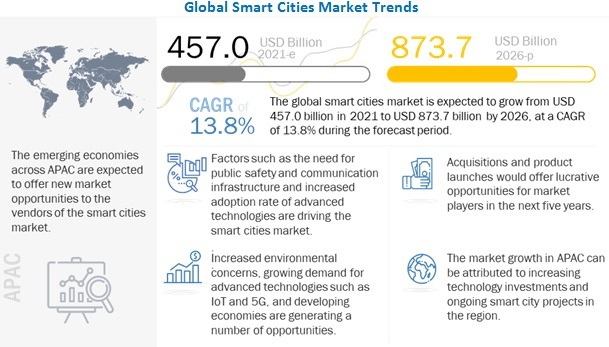
\includegraphics[width=.85\textwidth]{/02market_research/smart_cities_market}
	\caption{Global smart cities market trends.}
	\label{fig:smart_city_growth}
\end{figure}

\clearpage

As one can see, in figure \ref{fig:smart_city_growth}, according to MarketsandMarkets \cite{smart_cities_market} global smart cities market is expected to grow from USD 457 billion in 2021 to USD 873.7 billion by 2026, at a \ac{cagr} of 13.8\%, during the forecast period. Growing urbanization, need for efficient management and utilization of resources, and also the increasing demand for a healthy environment with efficient energy consumption are expected to be the major factors driving the growth of the smart cities market.

As figure \ref{fig:smart_cities_sols} shows, there are various applications of \ac{iot} technology for smart cities. In this project it will be created a solution that comprises Smart Lighting management and Smart Parking.

\begin{figure}[ht]
	\centering
	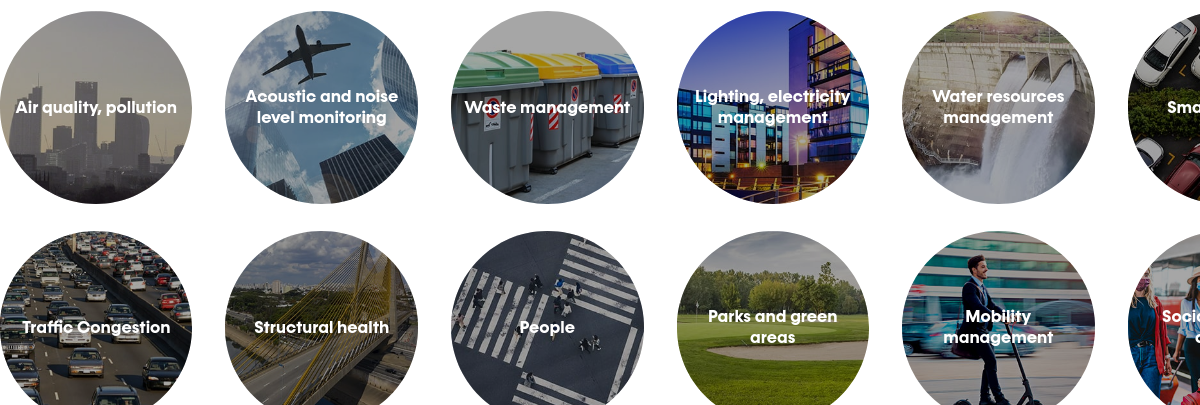
\includegraphics[width=1\textwidth]{/02market_research/applications_for_smart_cities}
	\caption{Applications of \ac{iot} technology for Smart Cities. \cite{smart_cities_solutions}}
	\label{fig:smart_cities_sols}
\end{figure}

\subsection{Smart Lighting}
Smart Street lighting is a rapidly growing lighting market, with an expected \ac{cagr} of 20.4 \% until 2026 \cite{smart_light_market}, implementing a smart management of public lighting to optimize energy consumption according to lighting needs. This is boosted by regulatory policies that encourage energy efficiency, \ac{iot} convergence and the drop of \ac{led} prices. This new concept of smart light post is also growing, implementing not only the smart management of street lights, but also features that go from basic \ac{led} replacement control, to traffic and video monitoring, environmental monitoring, and others.

\subsubsection{Telensa - PLANet}
Nowadays, Telensa is the market share leader in smart street lighting with more than ten years of experience.\cite{telensa} PLANet is an intelligent street lighting system, consisting of wireless nodes connecting individual lights, a dedicated network owned by the city and a central management application, seen in figure \ref{fig:telensa}. This system reduces energy and maintenance costs associated with street lighting and also improves quality of maintenance through automatic fault reporting.

\begin{figure}[ht]
	\centering
	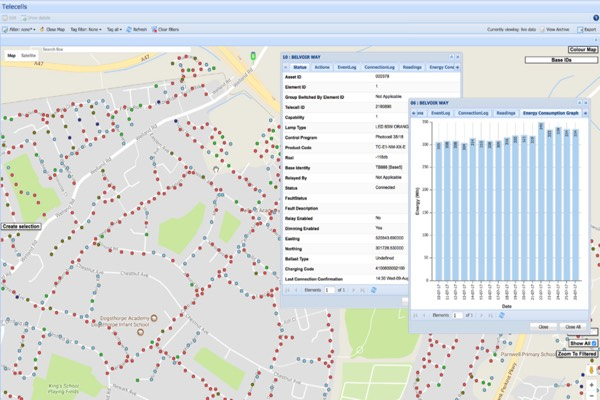
\includegraphics[width=0.8\textwidth]{/02market_research/telensa}
	\caption{Telecells - PLANet's Central Management System.}
	\label{fig:telensa}
\end{figure}

\subsubsection{FLASHNET - inteliLIGHT}
FLASHNET is a company focused on developing intelligent systems for smarter cities and better infrastructures and have created a solution that provides the right amount of light where and when needed to lighten the streets, the inteliLIGHT \cite{inteli_light}.

Using the existing infrastructure, this solution saves money and transforms the existing distribution level network into an intelligent infrastructure of the future, as shown in figure \ref{fig:intelilight}. Furthermore, the system is integrated with major \ac{iot} platforms and provides \ac{api} connectivity with City Management applications, ensuring compatibility with existing smart lighting and smart city initiatives.

\begin{figure}[ht]
	\centering
	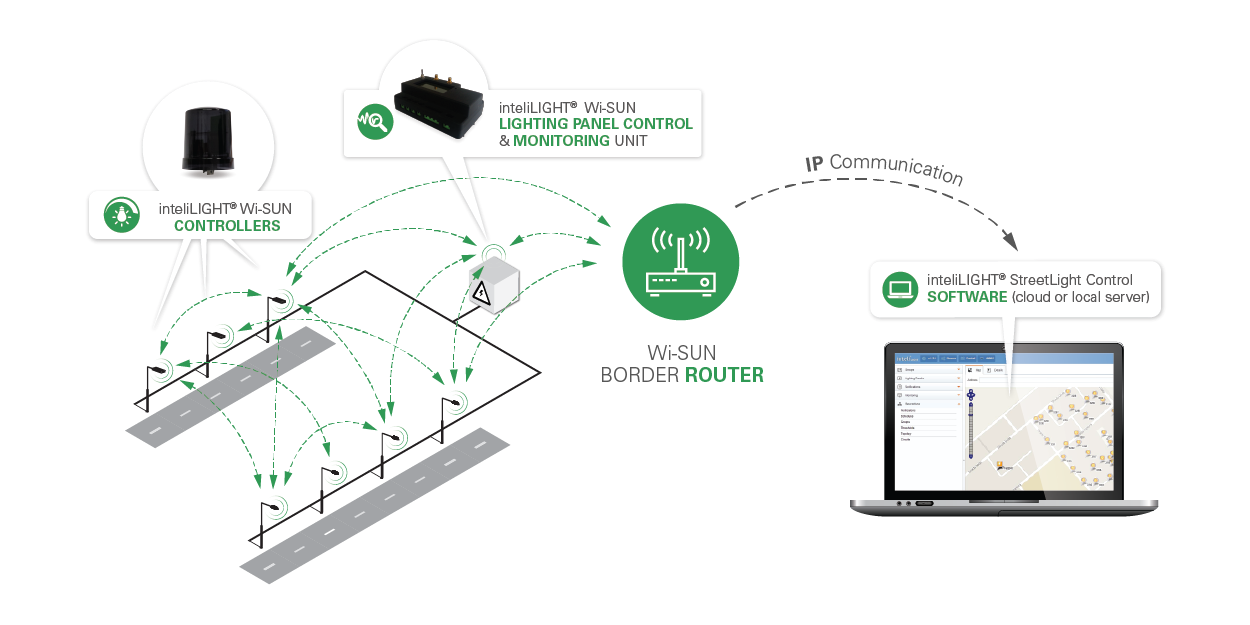
\includegraphics[width=0.95\textwidth]{/02market_research/intelilight}
	\caption{inteliLIGHT Communication Technology.}
	\label{fig:intelilight}
\end{figure}

\subsection{Smart Parking}
Smart parking, through the monitoring of parking spaces availability in the city, is also a growing market, expected to grow with a \ac{cagr} of 17.85\% in the forecast period of 2021 to 2028.\cite{smart_parking_market} The rise in investment in building driverless vehicles and an increase in the government’s initiative in building smart cities across the globe, along with the demand and adoption of \ac{iot} technology, are the main driving factors for the growth of smart parking market.

\subsubsection{intuVision - intuVision VA Parking}
Regarding only to the detection of available parking spaces, there is a solution, by intuVision, named intuVision VA Parking, which provides parking lot analytics to determine vehicle count and security, and monitor parking space availability at all times, both for cities and for private parking lots, as one can see in the figure \ref{fig:intuvision}.\cite{parking}

\begin{figure}[ht]
	\centering
	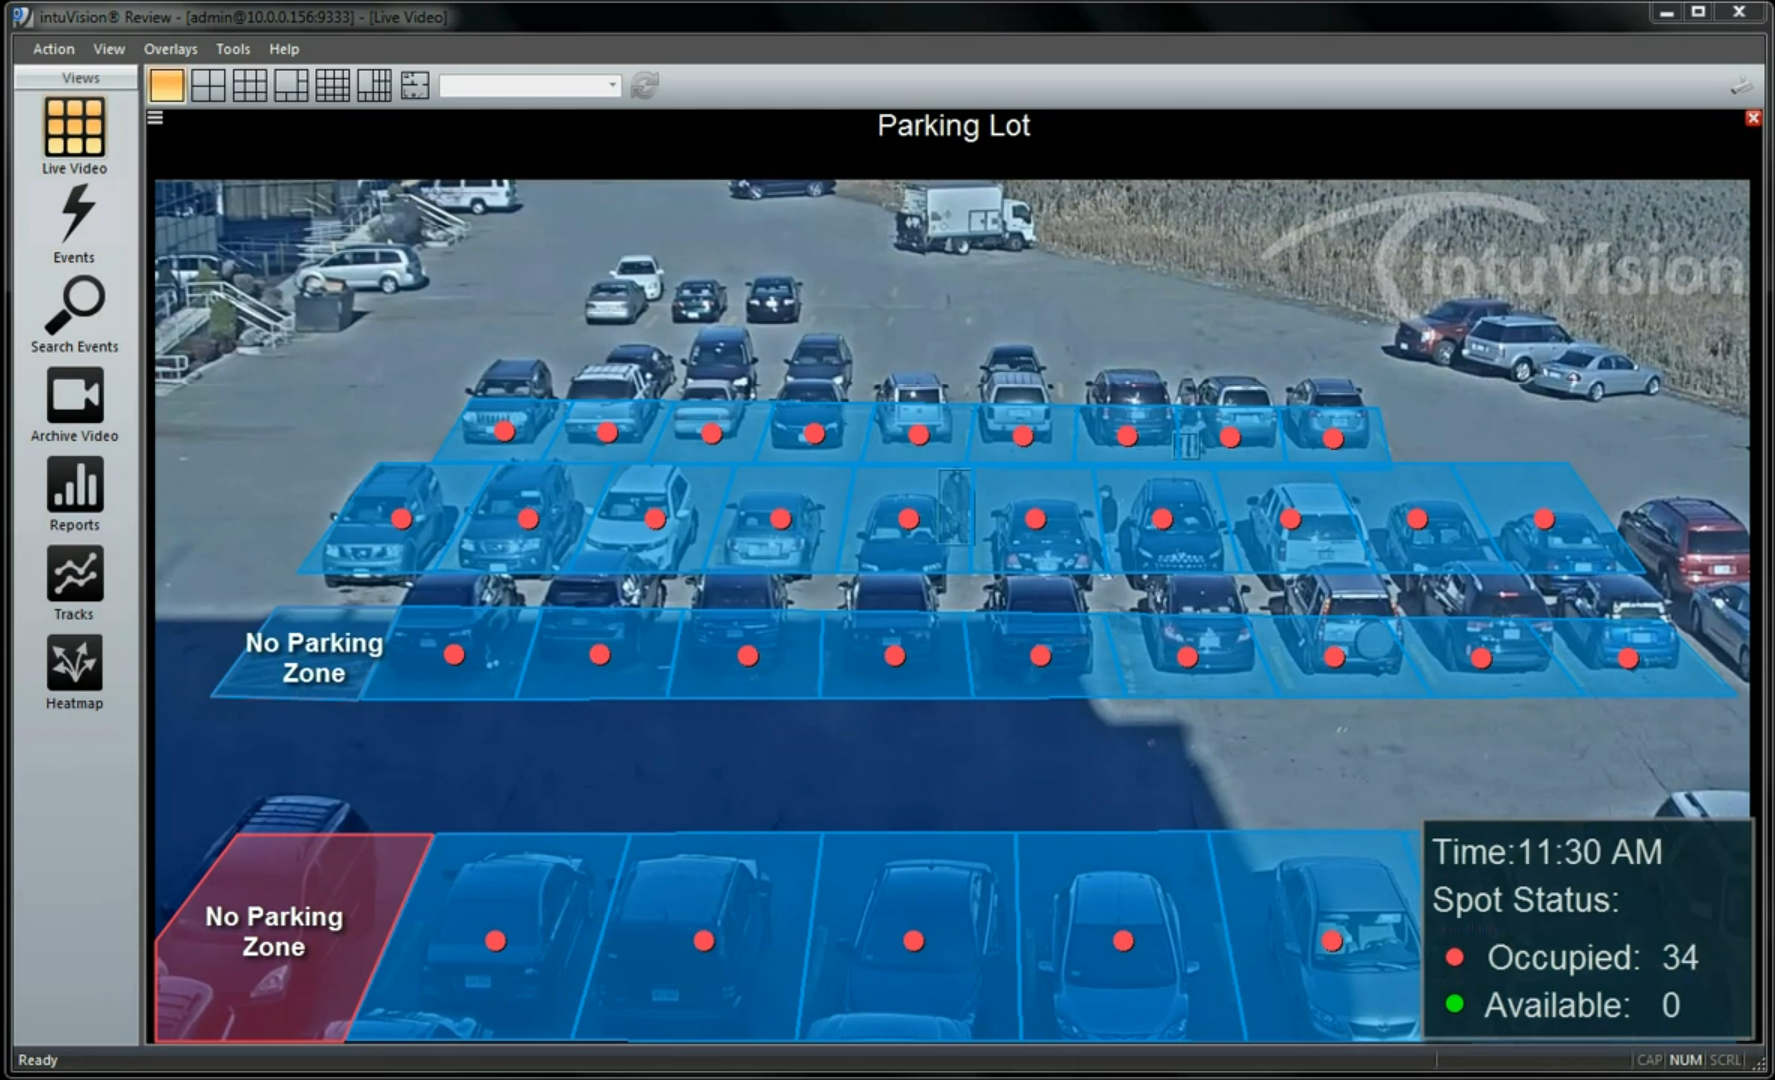
\includegraphics[width=0.8\textwidth]{/02market_research/intuvision}
	\caption{intuVision Parking Lot Demonstration.}
	\label{fig:intuvision}
\end{figure}

\section{Why choose our product}
This product aims to decrease power consumption associated with the traditional street light network, and also, using that infrastructure, contribute to the development of a smart city, detecting available parking spaces in the streets. This street lighting solution can be used in residential areas, public spaces or a large outdoor parking lot, feasible of being installed in existent lamp posts, requiring minimum changes to the original infrastructure. Although in this project it is not implemented, aside the parking spaces availability detection, this product can have the ability to monitor and to process various areas of interest using the camera built in, like for example, security purposes.


% ---------- SYSTEM ----------
\chapter{System}

% System Requirements and constraints
\section{System Requirements and Constraints}
\label{subsection:requirements_constraints}
In order for the system to have the desired performance, these requirements and constraints must be respected:
\subsection{Functional Requirements}
\begin{itemize}
	\item Sensors data acquisition;                          
	\item Motion detection;
	\item Control of a street lamp;
	\item Control a network of street poles;
	\item Wireless communication between local systems and gateway;
	\item Manage street poles network information through a mobile application;
	\item Empty parking spots detection;
	\item Add lamppost location through a mobile application;
	\item Access available parking spots location through a web site.
\end{itemize}

\subsection{Non-Functional Requirements}
\begin{itemize}
	\item User friendly mobile application and web site;
	\item Ambient luminosity sensing;
	\item Lower power consumption than actual street lights;
	\item Soft Real-Time Embedded System.
\end{itemize}

\subsection{Technical Constraints}
\begin{itemize}
	\item Buildroot
	\item C and C++ 
	\item Device Drivers
	\item Linux
	\item Raspberry Pi
	\item \ac{cps}
	\item Makefiles
	\item Pthreads
\end{itemize}

\subsection{Non-Technical Constraints}
\begin{itemize}
	\item Two members team
	\item Project deadline at the end of the semester
	\item Low budget
\end{itemize}

% Network Architecture
\section{Network Architecture}
The system to be developed is inserted in a network, more specifically, an infrastructure based network, as shown in figure \ref{fig:infr_based_arch}. This type of networks are composed by wireless segments of a more extensive network, whose core is usually a wired network. Infrastructure-based networks have a special station, called an \ac{ap} or \ac{bs}, which serves as an interface between the wireless segment and the rest of the network. Inside the wireless segment, there will be a centralized communication, so that all messages that circulate on the network pass through a central station. That way, the network only supports two transmission directions: the downward direction (downlink), from the base station to the other stations, and the uplink direction, from the stations to the base station. The downlink usually allows the simultaneous transmission of information to a group of stations in the cell (multicast) or to all stations (broadcast).

\begin{figure}[ht]
	\centering
	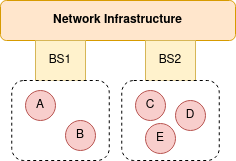
\includegraphics[width=.36\textwidth]{/03system_overview/infrastructure_based}
	\caption{Infrastructure based network architecture.}
	\label{fig:infr_based_arch}
\end{figure}

Street lighting is generally divided into sectors, facilitating maintenance and problem solving regarding the lighting network. In figure \ref{fig:network_arch}, one can see that the base station is a “special station”, since it connects the local network of lighting poles to other base stations, through a remote server, and also because it has a camera for the detection of available parking spaces. The rest of the stations that compose the local network, the local systems, will only do the smart management of their lamps.

\begin{figure}[ht]
	\centering
	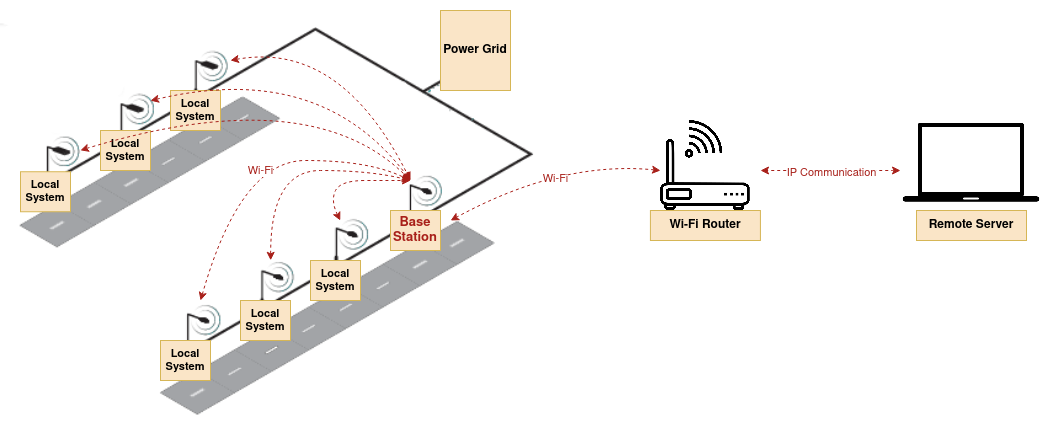
\includegraphics[width=1\textwidth]{/03system_overview/network_arch}
	\caption{Network architecture.}
	\label{fig:network_arch}
\end{figure}

The range of a Wi-Fi network depends primarily on the number and type of wireless access points used to build it, and so, the cost to build and maintain these networks increases significantly as the range increases.

The Wi-Fi signal range of any given access point also varies significantly from device to devices, depending on the specific 802.11 protocol that its used, the strength of its device transmitter and the nature of physical obstructions or radio interferences in the surrounding area. Also, due to laws of physics, 5 GHz Wi-Fi connections are more susceptible to obstructions than are 2.4 GHz. Generally, Wi-Fi routers operating on the traditional 2.4 GHz band reach up to 46 meters indoors and 92 meters outdoors. \cite{wi_fi_range}

Using a router running 802.11n, in open space the wi-fi signal range can be a little over 60 meters. \cite{wi_fi_802_11n} That being said, if each lamppost is spaced by 4 meters, each base station can easily connect with 10 local systems. To communicate with a remote server, the router will be connected to the internet through an Ethernet cable, or similar, that will most certainly already exist near the lampposts, in the telecommunications infrastructure.



\clearpage
% System Overview
% System architecture
\subsection{System Overview}
Through the system overview diagram, in figure \ref{fig:system_overview}, it is possible to identify the main modules of the system to be developed, and how they interact. We can divide the system into two subsystems: the local system, which represents a lamp post, and the remote system, that allows interaction with the system users.

\begin{figure}[ht]
	\centering
	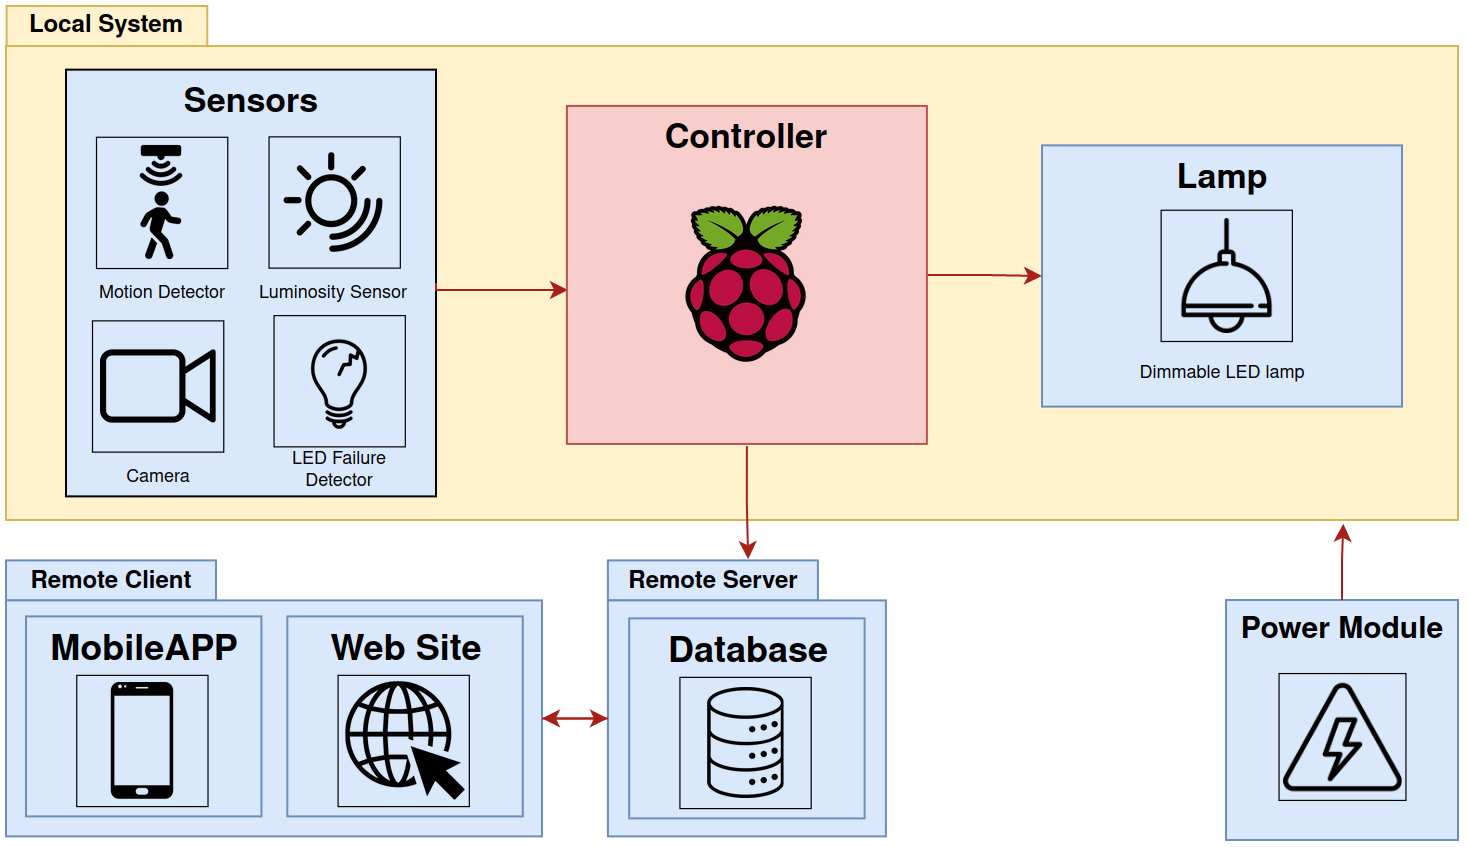
\includegraphics[width=1\textwidth]{system_overview}
	\caption{System Overview Diagram.}
	\label{fig:system_overview}
\end{figure}

The local system is composed of sensors, a controller and a lamp. Regarding the sensors, there will be a motion detector, to allow the detection of movement in the vicinity of the pole, a luminosity sensor, to detect the light conditions of the pole’s surroundings, a camera to find empty parking spots and a LED failure detector to know if the LED lamp is working. The controller, through sensors information, controls the luminosity of the lamp and communicates through the internet with a remote server, via Wi-Fi connection. 
The remote server consists of a database that stores all information about each lamp post location and operating status. This information can be accessed through a mobile application by the operator  responsible for the street lights network, in order to carry out the necessary maintenance of the lamp of each pole. Furthermore, the operator when installing a new lamp post can add its location to the database, using the mobile application. In addition, the database stores information on available parking spaces. When a user, a car driver, wants to know where there are empty parking places, he can access a website that informs him of the location of the empty parking spaces. \textbf{Knowing that the public lighting network is directly related to the electrical network, this will be used to power the local systems.}

\subsection{System Requirements and Constraints}
In order for the system to have the desired performance, these requirements and constraints must be respected:

\subparagraph{Functional Requirements}
\begin{itemize}
	\item Sensors data acquisition				
	\item Motion detector
	\item Control of a street lamp
	\item Wi-Fi communication
	\item Empty parking spots detection
	\item Manage system information through a mobile application
	\item Add lamp post location through a mobile application
	\item Access available parking spots location through a web site
\end{itemize}

\subparagraph{Non-Functional Requirements}
\begin{itemize}
	\item User friendly mobile application and web site
	\item Ambient luminosity sensing
	\item Lower power consumption than actual street lights
	\item Soft Real-Time Embedded System
\end{itemize}

\subparagraph{Technical Constraints}
\begin{itemize}
	\item Buildroot
	\item C and C++ 
	\item Device Drivers
	\item Linux
	\item Raspberry Pi
	\item \ac{cps}
	\item Makefiles
	\item Pthreads
\end{itemize}

\subparagraph{Non-Technical Constraints}
\begin{itemize}
	\item Two members team
	\item Project deadline at the end of the semester
	\item Low budget
\end{itemize}

\section{System Architecture}
Using the system overview diagram information, one can describe the system in two different architectures. Hardware architecture, as how the hardware modules interfaces with itself, and what are the physical components of the system, and software architecture, which details how the information is processed among different software layers.

\subsection{Hardware Architecture}
In figure \ref{fig:hw_arch}, one can see the diagram that represents the physical connections of the system. The power of most system components will be the output of the DC/DC converter, powering the controller and its associated sensors. In order to power the lamp and at the same time control its brightness, a driver must be used, taking the controller output and system power as inputs. The Raspberry Pi, despite not belonging to the local system, is powered similarly to the controller, via a DC/DC converter. Furthermore, it communicates with the controller wirelessly through its wireless interface, with the controller's wireless communication module.

\begin{figure}[ht]
	\centering
	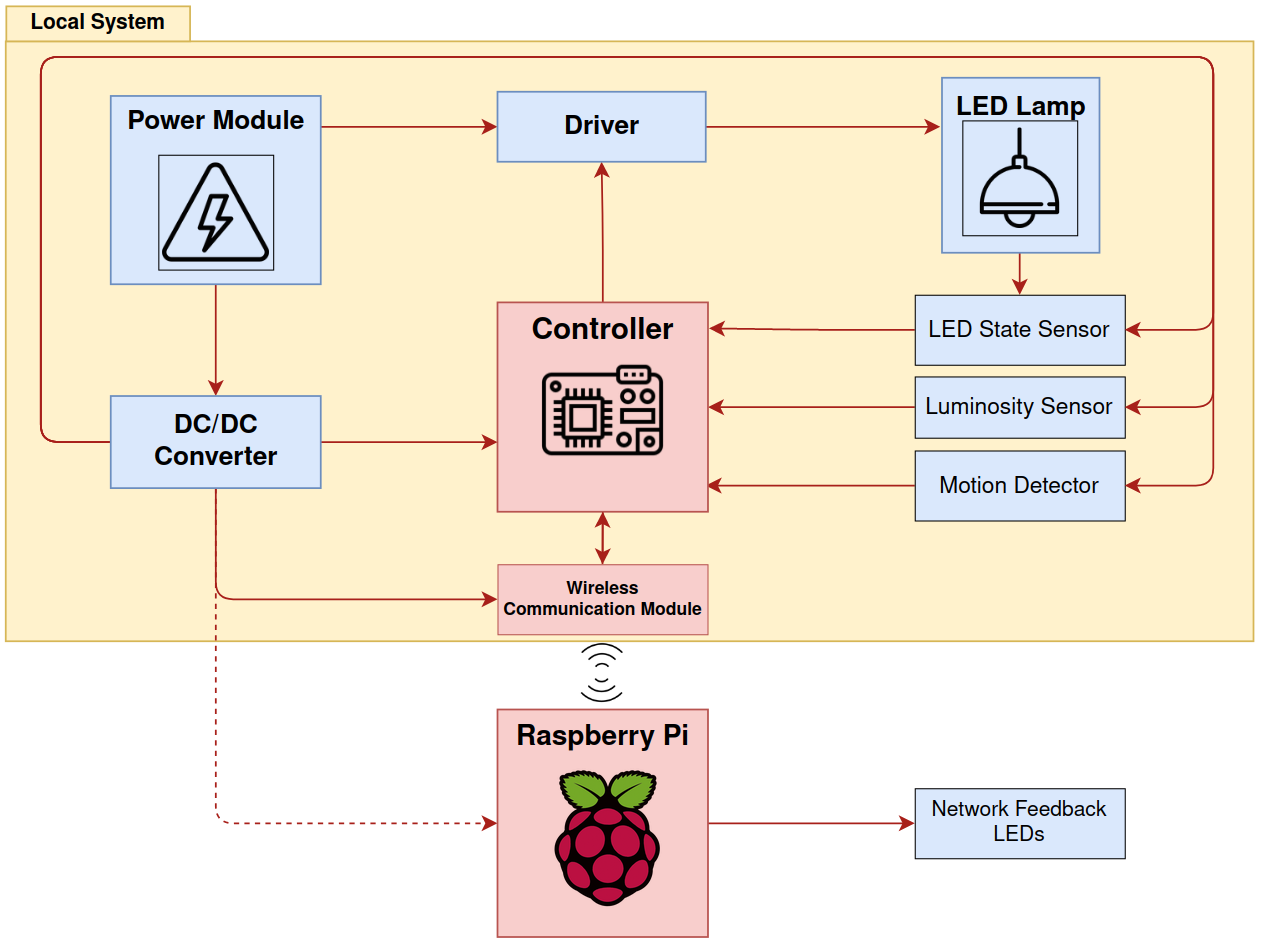
\includegraphics[width=1\textwidth]{hw_arch}
	\caption{Hardware Architecture Diagram.}
	\label{fig:hw_arch}
\end{figure}

\subsection{Software Architecture}
As seen previously, the system is divided into two subsystems: the local system and the monitoring system. Their software architectures are divided into three layers:

\begin{itemize}
	\item The Operating System layer, which is composed by the Operating System drivers and Board Support Packages;
	\item The Middleware layer, which includes software for abstracting the lower level layer packages. It works as a pipe since it links two applications, in different layers, so that data can be easily transmitted;
	\item The Application layer, where the core functionality of the program is built, with a resource for the API's in the lower level layers.
\end{itemize}

Regarding the local system, shown in figure \ref{fig:sw_arch_local}, the operating system layer is composed by the sensor drivers, such as the LED Failure Sensor, the Luminosity Sensor, the Motion Detector Sensor and also the Wireless Communication driver. As this system will acquire data from the environment through the mentioned sensors, at a low rate, and communicate this data to the monitoring device, multitasking will not be necessary, so this system will be bare metal, that is, it won’t have an operating system. In the middleware layer are the tools needed to acquire data from sensors and communicate wirelessly with the monitoring system. Finally, the communication between the different devices is managed in the application layer.

\begin{figure}[ht]
	\centering
	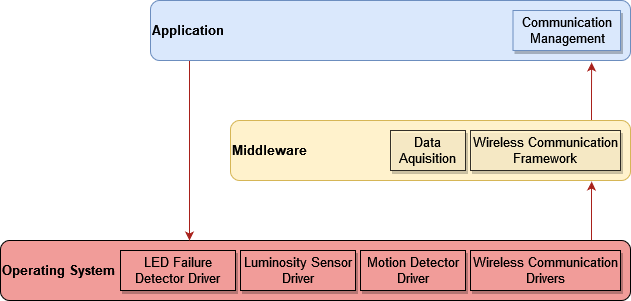
\includegraphics[width=1\textwidth]{sw_arch_local}
	\caption{Software Architecture Diagram - Local System.}
	\label{fig:sw_arch_local}
\end{figure}

Regarding the monitoring system, represented in figure \ref{fig:sw_arch_rasp}, the operating system layer is responsible for the network feedback LED drivers and for the wireless communication driver. This operating system will be a \ac{rtos}, due to the need to respond to events in a certain period of time and also multitasking. In the middleware layer, there will be the PThreads execution model, for multitasking, as well as the wireless communication and data acquisition frameworks. The application layer manages the system database, as well as the graphical user interface and all communications with local systems.

\begin{figure}[ht]
	\centering
	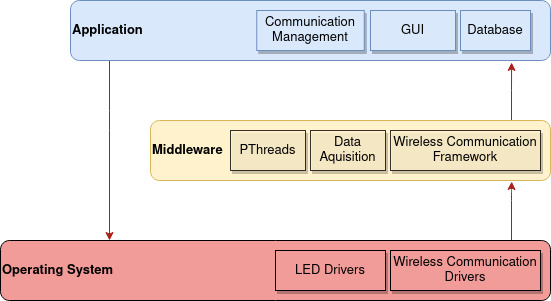
\includegraphics[width=1\textwidth]{sw_arch_rasp}
	\caption{Software Architecture Diagram - Monitoring System.}
	\label{fig:sw_arch_rasp}
\end{figure}


% ---------- SYSTEM ANALYSIS ----------
\chapter{System Analysis}

\section{Local System}
The local system's analysis is very similar to the base station analysis. Comparing to the base station, this system doesn't implement the parking spaces detection, since it doesn't have a camera, and only communicates with the base station. As in the base station, one can say that this is a passive system since it is most of the time waiting for something to happen.

\subsection{Events}
Listed in the table below, table \ref{table:ls_events}, are the main events that will occur in the local system and will affect its behavior. 

\begin{table}[h]
	\centering
	\resizebox{\columnwidth}{!}{
	\begin{tabular}{||c | c | c | c||} 
		\hline
		\textbf{Event} & \textbf{System Response} & \textbf{Source} & \textbf{Type}\\
		\hline\hline
Luminosity detector OFF & Power the lamp & Environment & Asynchronous\\\hline
LED failure detector ON & Notify remote system & Local system & Asynchronous\\\hline
Motion detected & Turn on the lamp & User & Asynchronous\\\hline
Requested to turn on the lamp & Turn on the lamp & Base station & Asynchronous\\\hline
Sensors data acquisition & Sample sensor values & Timer & Synchronous\\\hline
Update system information & Send data to remote system & Base station & Asynchronous\\
		\hline
	\end{tabular}
	}		
	
	\caption{Local system events.}
	\label{table:ls_events}
\end{table}

\subsection{Use Cases}
The local system use cases are represented on figure \ref{fig:ls_use_cases}. Like the base station, a street passerby, can interact with the local system by moving in the vicinity of the lamppost, triggering it's motion detector.

When movement is detected, the lamp is turned on and requests the base station to turn on the local system's neighbor lampposts. At the same time, the information that the lamppost was activated is sent to the base station, for this to be sent to the remote system.

Also, the local system can be asked, by the base station, to turn on its lamp.
\clearpage

\begin{figure}[ht]
	\centering
	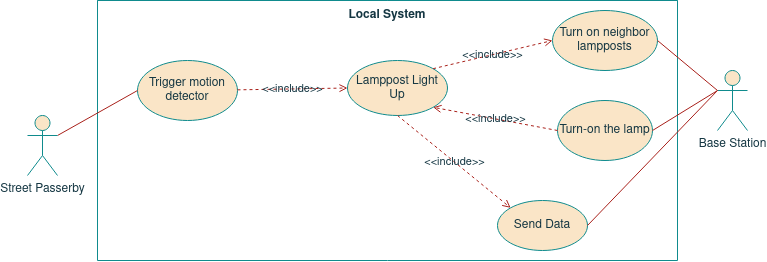
\includegraphics[width=1\textwidth]{/04local_system/LS_UseCase}
	\caption{Local system use cases.}
	\label{fig:ls_use_cases}
\end{figure}

\subsection{State Chart}
In figure \ref{fig:ls_state_chart} is represented the state chart of the local system. After the system configuration, which initializes the Wi-Fi communication management, sensors data acquisition, the system enters an idle state. To do the sensors data acquisition, like in the base station, it is used a sample period, that periodically triggers the execution of the function “SampleSensors”, presented previously, in figure \ref{fig:sample_sensors}. When the local system is requested by the base station to turn on its lamp, the lamp is turned-on and a timeout is started (turn off time, as mentioned before). The lamppost status is then sent to the base station, in order to send it to the remote server.

\begin{figure}[ht]
	\centering
	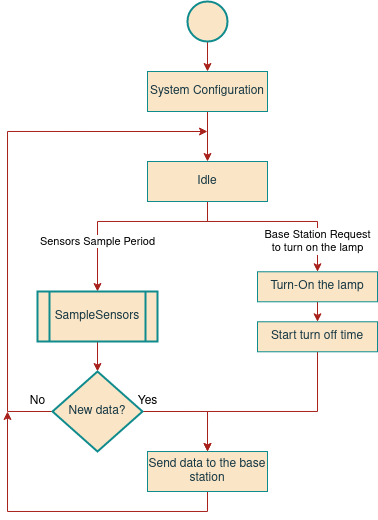
\includegraphics[width=.60\textwidth]{/04local_system/LS_StateChart}
	\caption{Local system state chart.}
	\label{fig:ls_state_chart}
\end{figure}

\clearpage
\subsection{Sequence Diagram}
The sequence diagram for the local system is represented in figure \ref{fig:ls_seq_diagram}. Again, this diagram is analogous to the one shown on the base station (figure \ref{fig:bs_seq_diagram}), having the differences that the local system only communicates with the base station, so any request that the local system wants to make to another local system has to go through the base station, and, due to that, the local system doesn't have the power to request another local system to turn its lamp on.

\begin{figure}[ht]
	\centering
	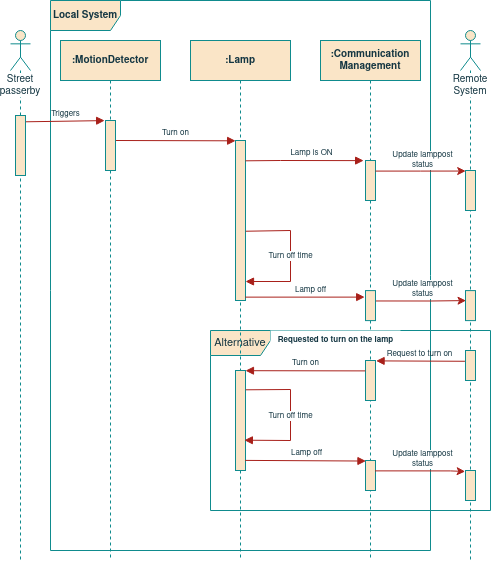
\includegraphics[width=.95\textwidth]{/04local_system/LS_SeqDiagram}
	\caption{Local system sequence diagram.}
	\label{fig:ls_seq_diagram}
\end{figure}

\clearpage
\section{Remote System}
\subsection{Events}

\begin{table}[ht]
	\centering
	\resizebox{\columnwidth}{!}{
	\begin{tabular}{||c | c | c | c||} 
		\hline
		Event & System Response & Source & Type\\
		\hline\hline
Login & Show application main screen if successful & Operator & Asynchronous\\\hline
Obtain geolocation & Request device geolocation & Mobile device & Asynchronous\\\hline
App notification & Notifies the operator about the lamppost status & Remote Server & Asynchronous\\\hline
Register operator & Add operator information to databas & Operator & Asynchronous\\\hline
Modify lamppost & Update lamppost information to database & Operator & Asynchronous\\\hline
Register lamppost & Add lamppost information to database & Operator & Asynchronous\\\hline
Insert location	& Show parking spots & User & Asynchronous\\\hline
Obtain geolocation & Request device geolocation & Mobile Device & Asynchronous
		\\\hline
	\end{tabular}
	}
		
	\caption{Remote system events.}
	\label{table:data}
\end{table}


\subsection{Use Cases}

\subsection{State Chart}

\subsection{Sequence Diagram}

\clearpage
\section{Estimated Budget}
\begin{table}[ht]
	\centering
	
	\begin{tabular}{||c | c||} 
		\hline
		\textbf{Product} & \textbf{Price(€)}\\
		\hline\hline
		Raspberry Pi 4B & 63,50\\\hline
		Industrial power supply 12 V & 5,00\\\hline
		Video camera & 8,86\\\hline
		Motion detector & 4,60\\\hline
		Luminosity sensor & 1,69\\\hline
		LED lamp 12 V & 3,63\\\hline
		Driver (MOSFET) & 1,00\\\hline
		Basic Eletronic Components & 5,00\\\hline
		\hline
		\textbf{Total} & \textbf{93,28}\\\hline
	\end{tabular}
	\caption{Estimated budget.}
	\label{table:data}
\end{table}

% Task Division and Gantt Chart
\clearpage
% Task Division/Gantt
\section{Task Division and Gantt Chart}
In figure x, is represented the Smart Street Lighting project schedule in form of a Gantt chart.

\begin{figure}[ht]
	\centering
	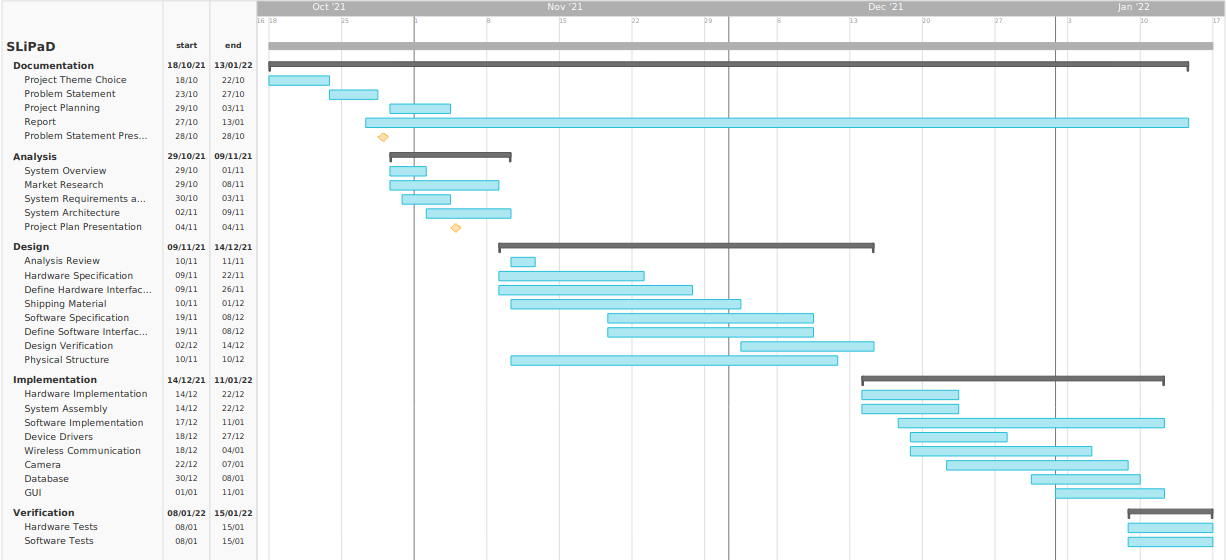
\includegraphics[width=1\textwidth]{Gantt_chart}
	\caption{Gantt chart.}
	\label{fig:Gantt_chart}
\end{figure}


% ---------- THEORICAL FOUNDATIONS ---------- 
\chapter{Theoretical Foundations}
In this chapter the theoretical foundations for the development of this project are presented, creating a solid groundwork for the design and implementation process.

\section{PThreads}
\section{Signals}
\section{PWM}

\section{Communication Protocols}
% assim tudo misturado aqui dentro?
\subsection{LoRaWAN}

\subsection{SPI}
\subsection{I2C}

\subsection{CSI}
%by way of a 15 Pin Ribbon Cable, to the dedicated 15-pin MIPI Camera Serial Interface (CSI), which was designed especially for interfacing to cameras. The CSI bus is capable of extremely high data rates, and it exclusively carries pixel data to the BCM2835 processor. 

\subsection{TCP-IP}
\subsection{HTTP}
\subsection{MQTT}

%********************************* DAEMONS *************************
\clearpage
\section{Daemons}
A daemon is a process that runs in the background and has no controlling terminal. The lack of a controlling terminal ensures that the kernel never automatically generates any job-control or terminal-related signals (such as SIGINT, SIGTSTP, and SIGHUP) for a daemon. \cite{linux_progr_interface}

A daemon is often created at system startup and runs until the system is shut down, being used to carry out specific tasks. It is a convention (not universally observed) that daemons have names ending with the letter d (example: \textit{httpd}, \textit{sshd}). 

Each process belongs to a process group, and the process group can contain one or more processes. There is a process leader in the process group, the \ac{pid} of the leader is the \ac{pgid}. More than one process group constitutes a "session". The process that establishes the session is the lead process for the session, and the \ac{pid} of the leader is the \ac{sid} of the session. Each process group in a session is called a "job". The meaning of a session is that multiple jobs can be controlled through one terminal, one foreground operation and the other running in the background. \cite{daemons}\newline

To become a daemon, a program performs the following steps:
\begin{enumerate}
	\item Perform a \textit{fork()}, after which the parent exits and the child continues.
	\item The  child  process  calls  \textit{setsid()} to  start  a  new  session  and  free itself of any association with a controlling terminal.
	\item Clear the process umask to ensure that, when the daemon creates files and directories, they have the requested permissions. (\textit{umask()})
	\item Change the process’s current working directory, typically to the root directory (\textit{chdir('/')}). This is necessary because a daemon usually runs until system shutdown, and if the daemon’s current working directory is on a file system other than the one containing '/', then that file system can’t be unmounted.
	\item Close  all  open file descriptors that the daemon has inherited  from its parent. (\textit{close()}) (A  daemon  may  need  to  keep  certain  inherited  file  descriptors  open,  so  this step  is  optional,  or  open  to  variation.)
\end{enumerate}

Since a daemon has no controlling terminal, the  \textit{syslog}  facility  provides  a  convenient  way  for  daemons  (and  other  applications)  to  log  error  and  other  messages  to  a  central  location.  These  messages  are processed by the \textit{syslogd} daemon, which redistributes the messages according to the dictates  of  the  syslogd.conf  configuration  file. 

Where appropriate, daemons should correctly handle the arrival of the SIGTERM and SIGHUP  signals. The  SIGTERM signal  should  result  in  an  orderly  shutdown  of  the daemon, while the SIGHUP signal provides a way to trigger the daemon to reinitialize itself by rereading its configuration file and reopening any log files it may be using.

%********************************* DEVICE DRIVERS *************************
\clearpage
\section{Device Drivers}
System memory in Linux can be divided into two distinct regions: kernel space and user space. Kernel space is where the kernel (the core of the operating system) executes and provides its services. User space is that set of memory locations in which user processes (everything other than the kernel) run. One of the roles of the kernel is to manage individual user processes within this space and to prevent them from interfering with each other. User processes can access kernel space only through the use of system calls, which are requests in a Unix-like operating system by an active process for a service performed by the kernel, such as input/output or process creation. \cite{kernel_space}

A device driver is a set of functions and data, in the kernel, that make the interface with an external I/O device. They are distinct “black boxes” that make a particular piece of hardware respond to a well-defined internal programming interface, hiding completely the details of how the device works. Devices  are  represented  by  entries  in  the  /dev  directory, being considered regular files.  Each  device  has  a  corresponding device driver, which implements a standard set of operations, including those  corresponding  to  the  \textit{open()},  \textit{read()}, \textit{ write()},  and  \textit{close()}  system  calls. \cite{linux_dev_drivers}

User activities are performed by means of a set of standardized calls that are independent of the specific driver. So the role of the device driver is to map those calls to device-specific operations that act on real hardware. Linux kernel offers a set of functions to the user space for the interaction with hardware, as one can see in the table \ref{table:device_driver}, in "User Functions". In the kernel space, Linux offers a set of functions that interact directly with the hardware and allows data transfer between kernel space and user space, as shown in "Kernel Functions".

\begin{table}[H]
	\centering
	\resizebox{\columnwidth}{!}
	{
		\begin{tabular}{|m{4cm}|m{3.5cm}|m{5cm}|}
			\hline
			\textbf{Event} & \textbf{User Functions} & \textbf{Kernel Functions}
			\\\hline\hline
			Load module & insmod & module\_init()
			\\\hline
			Remove module & rmmod & module\_exit()
			\\\hline
			Open module & fopen() & file\_operations: open
			\\\hline
			Read from device & fread() & file\_operations: read
			\\\hline
			Write to device & fwrite() & file\_operations: write
			\\\hline
			Close module & fclose() & file\_operations: close
			\\\hline
		\end{tabular}
	}
	\caption{Interface between an event, it's user function, and the kernel function called.}
	\label{table:device_driver}
\end{table}

When the kernel recognizes that a certain action were requested to a device, it calls an appropriate function from the driver, and transfers the process control from the user to the driver function. After the driver function ends its execution, it gives the control back to the user space process.

To associate the normal files to the kernel mode, the Linux system uses the major number and the minor number. Major number identifies the driver associated to the device and is normally used by Linux system to map I/O requests to driver code. Minor number is dedicated to internal use and it is used by kernel to determine exactly which device was reference. To do the association, it should be created a file or node in /dev directory, (calling \textit{mknod} as root user) that will be used to access the driver.

Linux supports three types of hardware devices: character, block and network device, being the character and block devices the most important. Character devices communicate directly with the user space program, so no buffer is required, for example the system’s serial ports. Block devices are accessed by the user space program by a system buffer, and can only be written and read from in multiples of the block size, typically 512 bytes. \cite{linux_progr_interface}

%********************************* IMAGE PROCESSING *************************
\clearpage
\section{Image Processing}
%Basically, an image is a two-dimensional array of pixels, so it can be represented in an cartesian coordinate system. 

Image processing consists of several techniques and methods used to manipulate images on a computer. The image processing helps improving the stored digital information, automate working with images and optimize image manipulation leading to efficient storage and transmission. Nowadays, image processing has many applications, like filtering images in editing apps and social media, medical technology, computer vision (objects identification, for example), pattern recognition, video processing and more. In this project, the image processing application is the computer vision, to detect available parking spots in the streets, using a camera.

In order to identify parking spots, one needs to find its outlines. The Canny Edge Detection \cite{canny} algorithm is a popular edge detection algorithm, and can be used to detect the parking spots outlines, providing an edge image. The canny edge detection is a multi-stage algorithm that goes through the stages: Noise reduction, Sobel Filtering, Non-maximum Suppression and Hysteresis Thresholding.

\myparagraph{Noise reduction}
The edge detection algorithm is sensible to noise in the image, so the first step is to remove the noise in the image using a 5x5 Gaussian filter. In figure \ref{fig:gaussian} one can see the results of the gaussian filter 5x5. 

\begin{figure}[H]
	\centering
	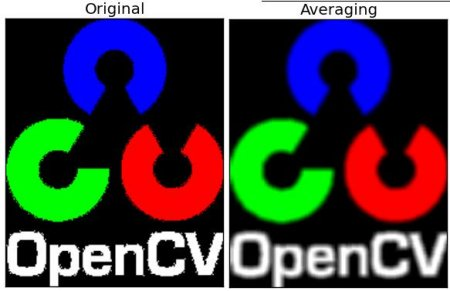
\includegraphics[width=.6\textwidth]{08theory/gaussian}
	\caption{Gaussian Filter Results.}
	\label{fig:gaussian}
\end{figure}

\myparagraph{Sobel Filtering}
Sobel filtering is an algorithm that finds intensity gradients on the image. This filter is applied in both horizontal and vertical direction, allowing to find the edge gradient and direction for each pixel. Figure \ref{fig:sobel}, shows the sobel filtering results.

\begin{figure}[H]
	\centering
	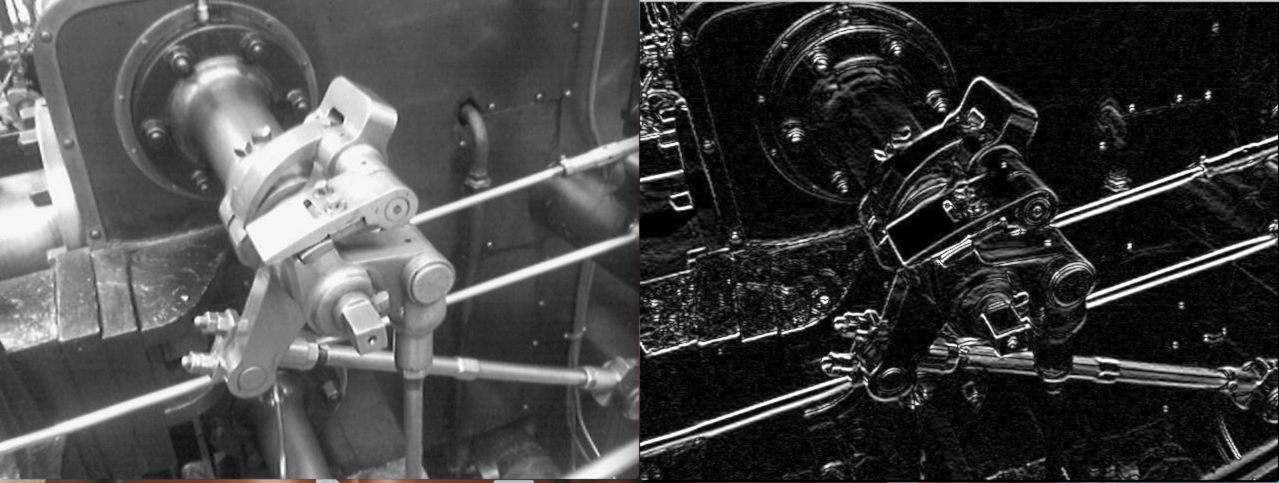
\includegraphics[width=.75\textwidth]{08theory/sobel}
	\caption{Sobel Filter Results.}
	\label{fig:sobel}
\end{figure}

\myparagraph{Non-maximum Suppression}
The non-maximum suppression algorithm does a full scan of the image in order to remove any unwanted pixels, that is, the pixels that don't constitute the edges of the image. In figure \ref{fig:nms}, one can see the non-maximum suppression algorithm. The point A is on the edge and the point B and C are in gradient directions. This algorithm suppresses the points B and C (put their pixel to 0) if they aren't a local maximum. If they are a local maximum, they are considered for the next stage as well as the point A.

\begin{figure}[H]
	\centering
	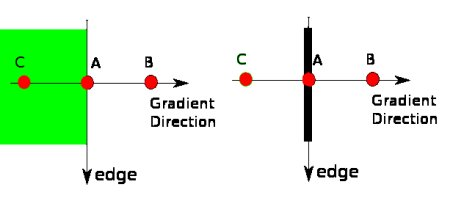
\includegraphics[width=.75\textwidth]{08theory/nms}
	\caption{Non-maximum Suppression Algorithm.}
	\label{fig:nms}
\end{figure}

\myparagraph{Hysteresis Thresholding}
This stage decides which edges considered until this point are really edges. This algorithm defines two threshold values, \textit{minVal} and \textit{maxVal}, in figure \ref{fig:hys_thr}. The edges that have an intensity gradient higher than \textit{maxVal} are considered edges and the edges that have lower intensity gradient than \textit{minValue}, aren't considered edges. The points with intensity gradient between this values are considered edges when they are connected to other edges with intensity gradient higher than \textit{maxVal} threshold value (the case of point C), and considered non-edges when they are not connected with other points with high intensity gradient value (the case of point B). 

\begin{figure}[H]
	\centering
	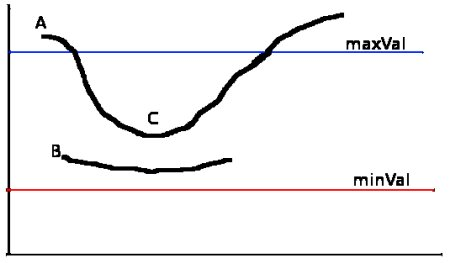
\includegraphics[width=.5\textwidth]{08theory/hys_thr}
	\caption{Hysteresis Thresholding Algorithm.}
	\label{fig:hys_thr}
\end{figure}

This algorithm, the Canny Edge Detection, allows the image processing algorithm to have only the strong edges of an image, being the final result represented in figure \ref{fig:canny}.

\begin{figure}[H]
	\centering
	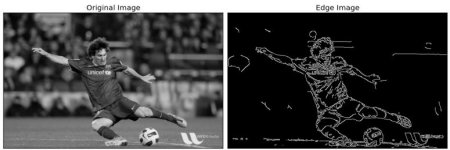
\includegraphics[width=.75\textwidth]{08theory/canny}
	\caption{Canny Edge Detection Result.}
	\label{fig:canny}
\end{figure}

\clearpage
\myparagraph{Hough Line Transform}

After detecting the edges of the image, one needs to take the processed image and use Hough Line Transform, which is an algorithm used to detect straight lines in an image. \cite{hough} 

Knowing that a parking spot is delimited by straight line edges, this algorithm provides the extreme coordinates of the parking spot outline. With the parking spots coordinates, one can make a parking map and knows where there are parking spots to after identify if the spot is occupied or not.

\myparagraph{Parking Spots Occupancy}




% ---------- SYSTEM DESIGN ----------
%\chapter{System Design}
\clearpage
\chapter{Hardware Specification}
\subsection{Development Board}

The development board for this project is the Raspberry Pi 4 Model B, shown in figure \ref{fig:rasp}, considering it is one of the constraints identified in the analysis phase (\ref{subsection:requirements_constraints}). This board includes a 64-bit quad-core ARM processor, the BCM2711, multimedia and connection features, ressembling to a computer-like board that serves multiple applications. The following list shows the Raspberry Pi 4 Model B main features:

\begin{itemize}
        \item 2GB LPDDR4-3200 SDRAM;
        \item 2.4 GHz and 5.0 GHz IEEE 802.11ac wireless, Bluetooth 5.0, BLE;
        \item Raspberry Pi standard 40 pin GPIO header;   
        \item 2 USB 3.0 ports and 2 USB 2.0 ports;
        \item 2 micro-HDMI ports;
        \item 1 display port (2-lane MIPI DSI);
        \item 1 camera port (2-lane MIPI CSI);
        \item 1 jack 3,5 mm port (4-pole stereo audio and composite video port);
		\item graphic support (OpenGL ES 3.1, Vulkan 1.0);
		\item Micro-SD card slot.
\end{itemize}

The Raspberry Pi 4 Model B is used as a development board for this project, as it would not be used in a final application because not all its features are used. So, in a final application, the development board would be chosen based on the features nedded or would be designed.

% A raspberry é apenas uma board de desenvolvimento, não é o hw que usariamos numa aplicação final.

\begin{figure}[H]
	\centering
	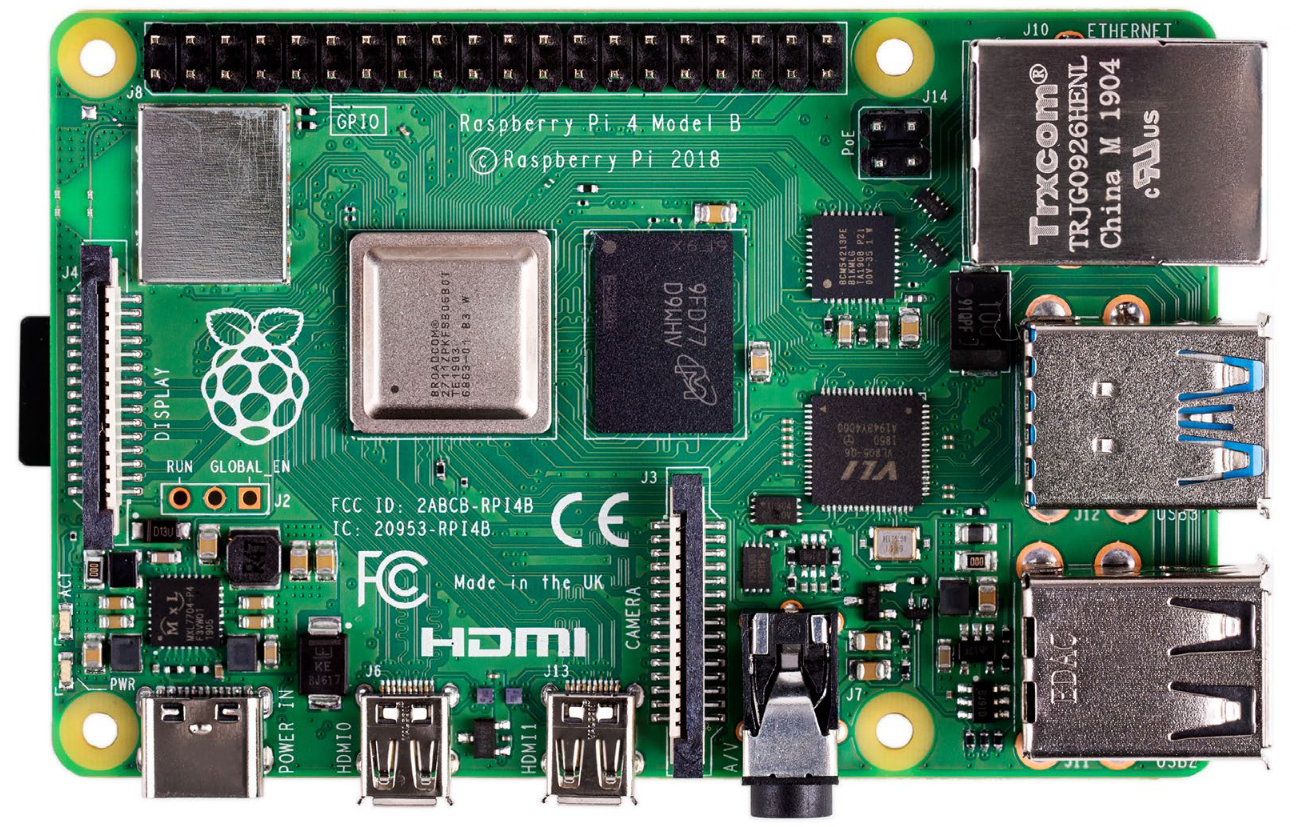
\includegraphics[width=.75\textwidth]{07hw_specification/raspberryPi}
	\caption{Raspberry Pi 4 Model B.}
	\label{fig:rasp}
\end{figure}

%**********************************************************
\myparagraph{\ac{gpio}}

The Raspberry Pi 4 Model B board comes with a standard 40 pin GPIO header, that allows to interface with external peripherals. This GPIO also provides some interface technologys, like UART, I2C or SPI. The GPIO pinout of this board is shown in figure \ref{fig:rasp_pinout} \cite{pinout}.

\begin{figure}[ht]
	\centering
	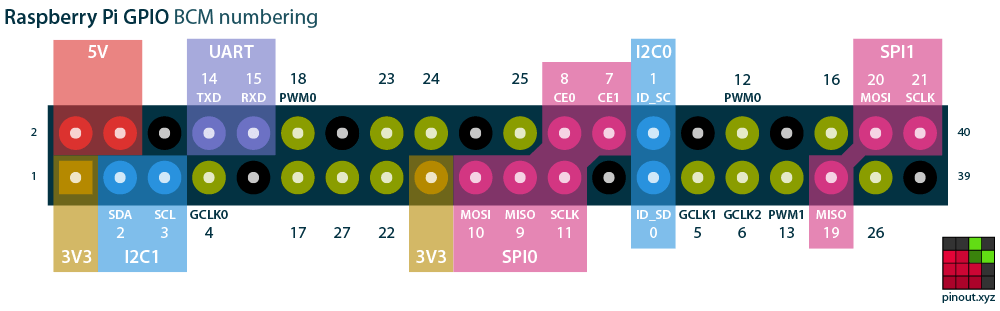
\includegraphics[width=1\textwidth]{07hw_specification/raspberryPi_pinout}
	\caption{Raspberry Pi 4 Model B GPIO Pinout.}
	\label{fig:rasp_pinout}
\end{figure}

%**********************************************************
\subsection{Lamp}

In order to light the streets efficiently, we use a LED lamp, that is the type of lamps with the better energy efficienty. It must be an adjustable lamp to control the lasmp brightness, so the lamp selected was a G4 socket 12 V AC/DC LED lamp. The lamp is controled using a driver, that is aproached in subsection \ref{subsection:driver} the that takes a \ac{pwm} signal (Pin 18) from the Raspberry Pi as input. 

\begin{figure}[ht]
	\centering
	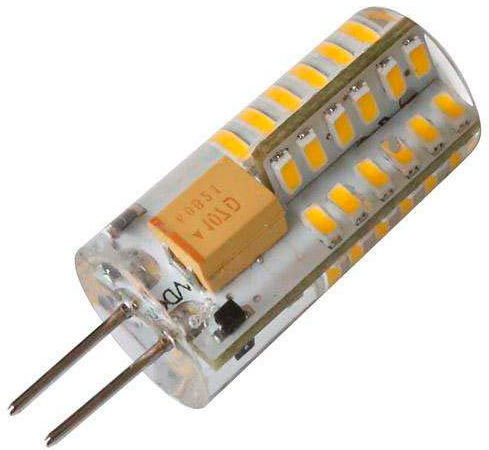
\includegraphics[width=1\textwidth]{07hw_specification/lamp}
	\caption{LED Lamp.}
	\label{fig:lamp}
\end{figure}

\myparagraph{Characteristics}

\begin{itemize}
	\item Power supply: DC 12 V;
	\item Eletric power: 2 W;
	\item Adjustable;
	\item Socket: G4;   
	\item Chip controller: SMD3014.
\end{itemize}

In a real-scale project, it would be used a different lamp, with supplu voltage of 230 V AC and other specific characteristics  like  rate, in  from water and dust (IP65 \ref{ip65}). It would be also used a LED lamp with higher eletric power. 

%**********************************************************
\subsection{Luminosity Sensor}

In order to know when is night time, that is, when the light conditions are low, one needs to determine the ambient light conditions. To do that, it is used a digital ambient light sensor, the TSL2581 \cite{light_sensor}, represented in \ref{fig:light_sen}. It was chosen this project because this sensor communicates with the Raspberry Pi using \ac{i2c} communication protocol, so it gives a digital value of the lumminusity, according to the light conditions, so it isn't necessary to calibrate this sensor (with a potenciometer, for example) when installing a new local system.

\begin{figure}[ht]
	\centering
	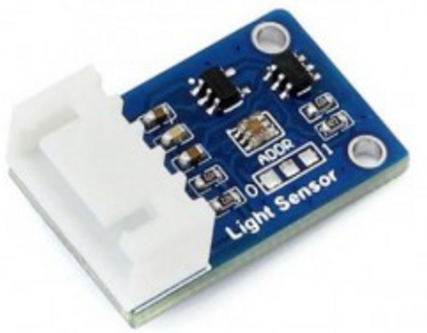
\includegraphics[width=0.60\textwidth]{07hw_specification/light_sen}
	\caption{TSL2581 Light Sensor.}
	\label{fig:light_sen}
\end{figure}

\paragraph*{Characteristics}
\begin{itemize}
	\item \ac{i2c} interface directly outputs the ambient light intensity value;
	\item High precision output, with an infrared photodiode;
	\item Allows connection to 3,3 V or 5,5 V MCU systems;
	\item 16-bit resolution.
\end{itemize}

In the table \ref{table:light_sen} is shown the TSL2581 interface pins, being the \textit{SDA} pin used for data transfer, the \textit{SCL} pin used for clock synchronisation and the \textit{INT} pin used for interrupt output. 

\begin{table}[H]
	\centering
	\begin{tabular}{|m{5cm}|m{6cm}|}
		\hline
		\textbf{TSL2581 Pin} & \textbf{Board Pin}\\\hline\hline
		VCC & Pin 1 (3,3) V\\\hline
		GND & Pin 6 (GND)\\\hline
		SDA & Pin 2 (SDA)\\\hline
		SCL & Pin 3 (SCL)\\\hline
		INT & -\\
		\hline
	\end{tabular}		
	
	\caption{Light Sensor TSL2581 Interface Pins.}
	\label{table:light_sen}
\end{table}

\myparagraph{Test Cases}
It is important to know how the light sensor works, and how it will behave upon certain events. In table \ref{table:test_light_sen} are shown test cases to this module.

\begin{table}[H]
	\centering
	\resizebox{\columnwidth}{!}
	{
		\begin{tabular}{|m{3cm}|m{5cm}||m{5cm}|}
			\hline
			\textbf{Test Case} & \textbf{Expected Output} & \textbf{Real Output}
			\\\hline\hline
			Read ambient luminosity & Return ambient luminosity  & -
			\\\hline
		\end{tabular}
	}
	\caption{Test Cases: TSL2581.}
	\label{table:test_light_sen}
\end{table}

%**********************************************************
\clearpage
\subsection{Motion Detector}
To know when to turn on the light, it is necessary to detect movement in the streets. For this project it is used a motion detector, more specifically a \ac{pir} sensor. The chosen sensor for this purpose was the PIR HC-SR501 \cite{pir}.

\begin{figure}[H]
	\centering
	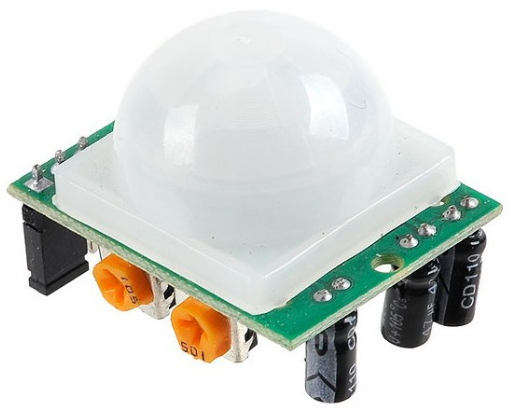
\includegraphics[width=0.70\textwidth]{07hw_specification/pir}
	\caption{PIR HC-SR501.}
	\label{fig:pir}
\end{figure}

\paragraph*{Characteristics}
\begin{itemize}
	\item Supply voltage range of 4,5 - 20 V;
	\item Static current: 50 uA;
	\item Detection range of 7 meters;
	\item Detection angle of 110 degrees;
	\item Two potenciometers to adjust the trigger sensitivity and the delay of the trigger signal, between 0,3 seconds and 5 minutes;
\end{itemize}

In the table \ref{table:pir} is shown the PIR HC-SR501 interface pins, being the output signal the pin SIGNAL. When no movement is detected, the sensor output is low (0,3~V), and when movement is detected, the sensor SIGNAL is high (5~V). 

\begin{table}[H]
	\centering
	\begin{tabular}{|m{5cm}|m{6cm}|}
		\hline
		\textbf{PIR HC-SR501 Pin} & \textbf{Board Pin}
		\\\hline\hline
		
		VCC & Pin 2(5 V)\\\hline
		SIGNAL & Pin 27\\\hline
		GND & Pin 6(GND)\\
		\hline
	\end{tabular}
	
\caption{PIR HC-SR501 Interface Pins.}
\label{table:pir}
\end{table}

\myparagraph{Test Cases}
It is important to know how the motion detector module works, and how it will behave upon certain events. In table \ref{table:test_pir} are shown test cases to this module.

\begin{table}[H]
	\centering
	\resizebox{\columnwidth}{!}
	{
		\begin{tabular}{|m{3cm}|m{5cm}||m{5cm}|}
			\hline
			\textbf{Test Case} & \textbf{Expected Output} & \textbf{Real Output}
			\\\hline\hline
			Movement in front of the sensor & Pin SIGNAL high (5 V) & -
			\\\hline
			No movement in front of the sensor & Pin SIGNAL low (0,3 V) & -
			\\\hline
		\end{tabular}
	}
	\caption{Test Cases: PIR HC-SR501.}
	\label{table:test_pir}
\end{table}

%**********************************************************
\subsection{Lamp Failure Detector}
In order to know when the lamp is broken, one needs to use a lamp failure detector, so it was designed a circuit represented in figure \ref{fig:failure_circuit}. 
%When the lamp  

\begin{figure}[H]
	\centering
	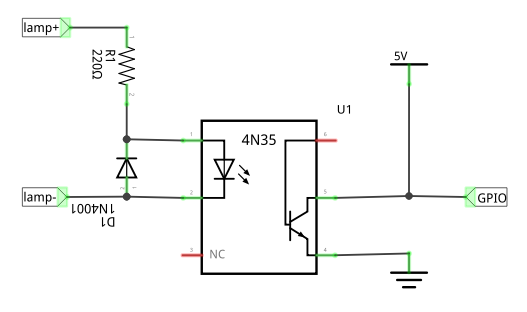
\includegraphics[width=0.6\textwidth]{07hw_specification/failure_schem}
	\caption{Lamp Failure Detector Circuit.}
	\label{fig:failure_circuit}
\end{figure}

The optocoupler chosen was the 4N35 \cite{4n35}, represented in figure \ref{fig:failure}

\begin{figure}[H]
	\centering
	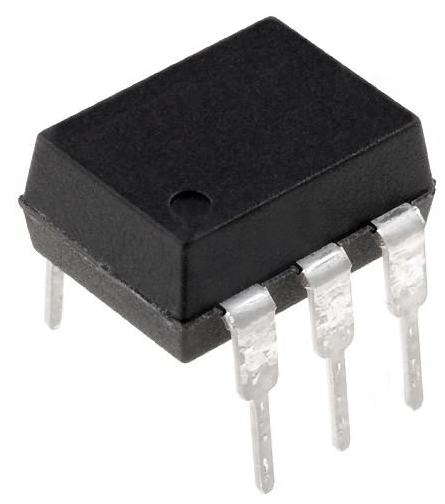
\includegraphics[width=0.4\textwidth]{07hw_specification/failure}
	\caption{Optocoupler 4N35.}
	\label{fig:failure}
\end{figure}

%**********************************************************
\subsection{Camera}
In order to the detection of available parking spots, it's used a camera, as shown in figure \ref{fig:camera}. This is the Raspberry Pi Camera Module V1, capable of delivering a clear 5 MP resolution image, or 1080p HD video recording at 30fps. \cite{camera}

\begin{figure}[H]
	\centering
	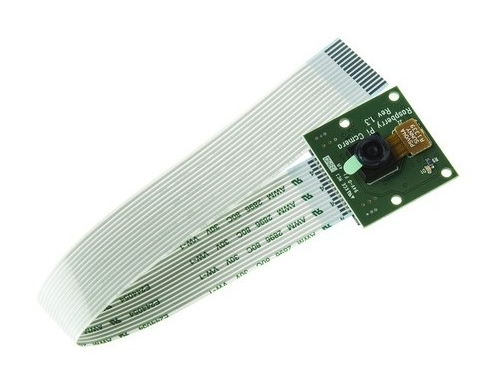
\includegraphics[width=0.6\textwidth]{07hw_specification/camera}
	\caption{Raspberry Pi Camera Module V1.}
	\label{fig:camera}
\end{figure}

\paragraph*{Characteristics}
\begin{itemize}
	\item 5MP OmniVision 5647 sensor;
	\item Fixed focus lens onboard;
	\item Still Picture Resolution: 2592 x 1944;
	\item 15-pin ribbon cable, to the dedicated 15-pin MIPI \ac{csi};
	\item Video recording: Supports 1080p @ 30fps, 720p @ 60fps.
\end{itemize}

\clearpage
\myparagraph{Connection scheme}
This device plugs directly into the \ac{csi} connector on the Raspberry Pi, as shown in figure \ref{fig:connect_camera}, through the use of a 15-pin ribbon cable.

\begin{figure}[ht]
	\centering
	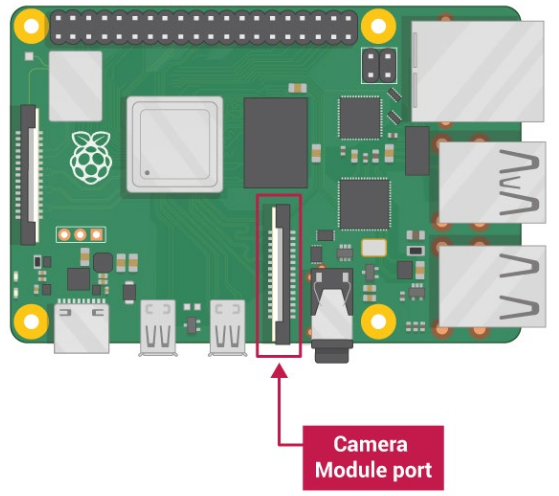
\includegraphics[width=0.60\textwidth]{07hw_specification/connect_camera}
	\caption{Connection scheme: Camera Module.}
	\label{fig:connect_camera}
\end{figure}

\myparagraph{Test Cases}
It is important to know how the camera module will behave upon certain events. In table \ref{table:test_camera} are shown test cases to this module.

\begin{table}[H]
	\centering
	\resizebox{\columnwidth}{!}
	{
	\begin{tabular}{|m{3cm}|m{5cm}||m{5cm}|}
		\hline
		\textbf{Test Case} & \textbf{Expected Output} & \textbf{Real Output}
		\\\hline\hline
		Take picture & Clear output image & -
		\\\hline
	\end{tabular}
	}
	\caption{Test Cases: Camera Module.}
	\label{table:test_camera}
\end{table}


%**********************************************************
\clearpage
\subsection{LoRa Module}
To allow each local system to communicate to the gateway, and vice-versa, it's used LoRa communication technology, requiring for that LoRa Modules, as the one presented in figure \ref{fig:lora_module}. This module, from Ai-Thinker company, uses SX1278 \ac{ic} from SEMTECH, and works on a 433~MHz frequency, with a range up to 10 km in line of sight. \cite{sx1278} \cite{lora_module}

\begin{figure}[H]
	\centering
	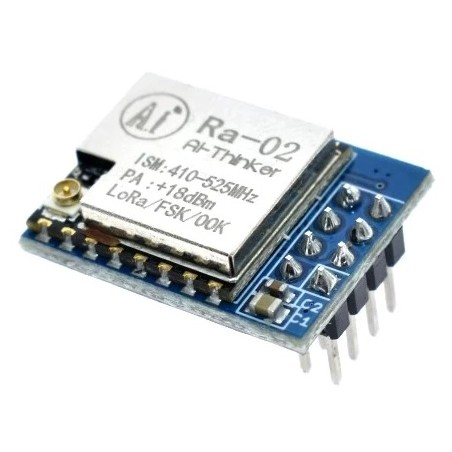
\includegraphics[width=0.5\textwidth]{07hw_specification/lora_module}
	\caption{LoRa Module SX1278 RA-02 433 MHz.}
	\label{fig:lora_module}
\end{figure}

\paragraph*{Characteristics}
\begin{itemize}
	\item LoRa modulation technology (Supports also FSK, GFSK, MSK, GMSK and OOK modulation modes);
	\item Effective Bitrate : 0,018 - 37,5 kbps;
	\item Payload length: 64 bytes;
	\item Half-duplex SPI communication;
	\item Programmable bit rates up to 300kbps;
	\item Packet engine with CRC up to 256 bytes;
	\item Male U.FL connector to support using of external RF antenna - Diameter: 15,5mm.
\end{itemize}

\begin{table}[H]
	\centering
		\begin{tabular}{|m{5cm}|m{6cm}|}
			\hline
			\textbf{SX1278 RA-02 Pinout} & \textbf{Description}
			\\\hline\hline
		
			VCC & Power in - 3,3 V\\\hline
			GND & Ground\\\hline
			RST & Reset \\\hline
			SCK & SPI clock input\\\hline
			NSS & SPI selected-IN\\\hline
			MISO & SPI data output\\\hline
			MOSI & SPI data input\\\hline
			DIO0 & Digital Input/Output Pin 0\\\hline
			\hline
		\end{tabular}
	
	\caption{LoRa Module SX1289 RA-02 Pinout Description.}
	\label{table:lora_module_pinout}
\end{table}

In order to achieve longer range and better signal quality in LoRa communication, an antenna may be used, as the one shown in figure \ref{fig:lora_antena}. RF antennas play a critical role in diverting, directing or concentrating radio wave transmission in a particular direction. 

%Antennas that have high gain will enable one to achieve longer range and better signal quality in LoRa communication, but must be aimed specifically in the direction of the receiving antenna. 

\begin{figure}[H]
	\centering
	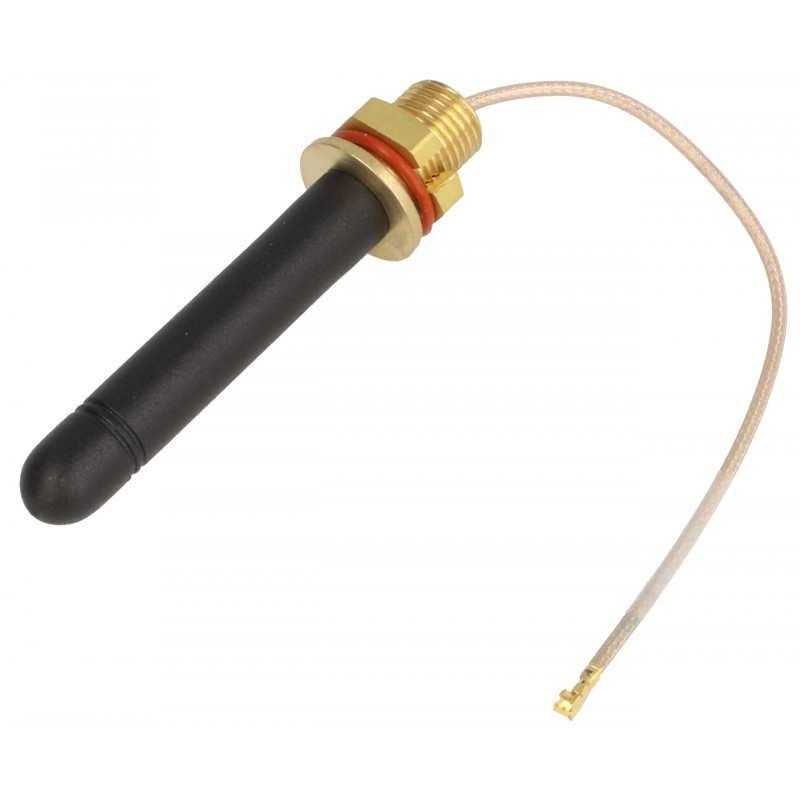
\includegraphics[width=0.40\textwidth]{07hw_specification/lora_antena}
	\caption{RF Antenna 433 MHz.}
	\label{fig:lora_antena}
\end{figure}

\paragraph*{Characteristics}
\begin{itemize}
	\item Frequency: 433,05 - 434,79 MHz;
	\item Antenna gain: 2 dBi;
	\item Connector I-PEX (U.FL) - Diameter: 15,5mm;
	\item Impedance 50 $\Omega$.
\end{itemize}

\myparagraph{Connection scheme}
In table \ref{table:connect_lora} it is shown the connection scheme of the LoRa module to the Raspberry Pi (remember figure \ref{fig:rasp_pinout}). Keep in mind that the RF antenna is directly connected to the LoRa module through an U.FL connector.

\begin{table}[H]
	\centering
	\begin{tabular}{|m{5cm}|m{6cm}|}
		\hline
		\textbf{SX1278 RA-02 Pin} & \textbf{Raspberry Pi Pin}
		\\\hline\hline
		
		VCC & 3,3 V
		\\\hline
		GND & GND
		\\\hline
		RST & GPIO 4
		\\\hline
		SCK & CLK
		\\\hline
		NSS & SPI0 CE0
		\\\hline
		MISO & SPI0 MISO
		\\\hline
		MOSI & SPI0 MOSI
		\\\hline
		DIO0 & GPIO 17
		\\\hline
	\end{tabular}
	
	\caption{Connection scheme: LoRa Module.}
	\label{table:connect_lora}
\end{table}

\myparagraph{Test Cases}
It is important to know how the LoRa module works, and how it will behave upon certain events. In table \ref{table:test_lora} are shown test cases to this module.

\begin{table}[H]
	\centering
	\resizebox{\columnwidth}{!}
	{
		\begin{tabular}{|m{3cm}|m{5cm}||m{5cm}|}
			\hline
			\textbf{Test Case} & \textbf{Expected Output} & \textbf{Real Output}
			\\\hline\hline
			Establish connection & Stable connection established & -
			\\\hline
			Send data & Data sent correctly & -
			\\\hline
			Receive data & Data received correctly & -
			\\\hline
		\end{tabular}
	}
	\caption{Test Cases: LoRa Module.}
	\label{table:test_lora}
\end{table}

%**********************************************************

\subsection{Driver}
\label{subsection:driver}
In order to control the lamp brightness through a GPIO pin from the Raspberry Pi, it's needed a driver circuit, as shown in figure \ref{fig:driver}. This circuit takes as input a \ac{pwm} signal, provided by the raspberry Pi, and also the power for the lamp, \(V_{CL}\), which comes directly from the power supply 12 V \ac{dc} output of the power module. The output of this circuit, the lamp voltage \(V_{L}\), is directly related to it's brightness, which one wants to control.

\begin{figure}[H]
	\centering
	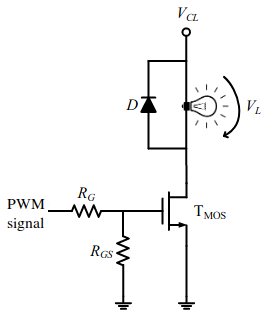
\includegraphics[width=0.5\textwidth]{07hw_specification/driver}
	\caption{Driver circuit to control lamp brightness.}
	\label{fig:driver}
\end{figure}

The \ac{pwm} signal only takes two values, 0 or 3,3 V, but its average value over time is varied, changing at high frequency the time intervals in which the transistor \(T_{MOS}\) is conducting (applied voltage 3,3 V) and at cutoff (applied voltage 0 V). So, as the \ac{pwm} duty cycle increases, the transistor conducts for more time, leading to an increase of \(V_{L}\), and, therefore, to an increase of the lamp brightness. In any case, the power dissipation in the transistor is very low, because of the rapid change between each transistor state, conducting (at saturation) or at cutoff.

\paragraph*{Characteristics}
\begin{itemize}
	\item Transistor MOSFET
\end{itemize}

\myparagraph{Connection scheme}

\myparagraph{Test Cases}
%**********************************************************

\subsection{Power Module}
As specified before, it's needed a power module to power the system, using the power grid. For that, it's necessary the use of an \ac{ac}/\ac{dc} power supply, in order to use the power grid electricity, which in Portugal is 230 V \ac{ac}. The power supply must provide 12 V \ac{dc}, as it is needed to power the lamp, as previously seen. The power supply used is shown in figure \ref{fig:power_supply}. \cite{power_supply}

\begin{figure}[H]
	\centering
	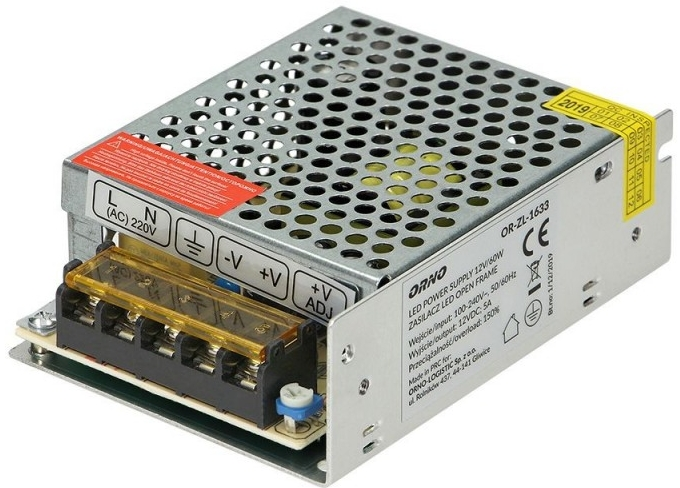
\includegraphics[width=0.5\textwidth]{07hw_specification/power_supply}
	\caption{ORNO Industrial Power Supply 12 V / 5 A.}
	\label{fig:power_supply}
\end{figure}

\paragraph*{Characteristics}
\begin{itemize}
	\item Input voltage: 100-240 V \ac{ac}, 60 W;
	\item Output voltage: 12 V \ac{dc};
	\item Output current: 5 A;
	\item Protected against overload, short circuit, over-voltage and over-heating.
\end{itemize}

\begin{table}[H]
	\centering
	\begin{tabular}{|m{5cm}|m{6cm}|}
		\hline
		\textbf{Power Supply Pinout} & \textbf{Description}
		\\\hline\hline
		 
		L & Power grid phase 230 V \ac{ac}
		\\\hline
		N & Power grid neutral
		\\\hline
		GND & GND
		\\\hline
		-V & Output -12 V \ac{dc}
		\\\hline
		+V & Output +12 V \ac{dc}
		\\\hline
	\end{tabular}
	\caption{Power Supply Pinout Description.}
	\label{table:power_supply_pinout}
\end{table}

For educational purposes, in this project the power supply will be connected to a power plug, and not directly connected with eletrical grid wires, being for that necessary a plug to bare end wire, as the one shown in figure \ref{fig:eletrical_wire}.

\begin{figure}[H]
	\centering
	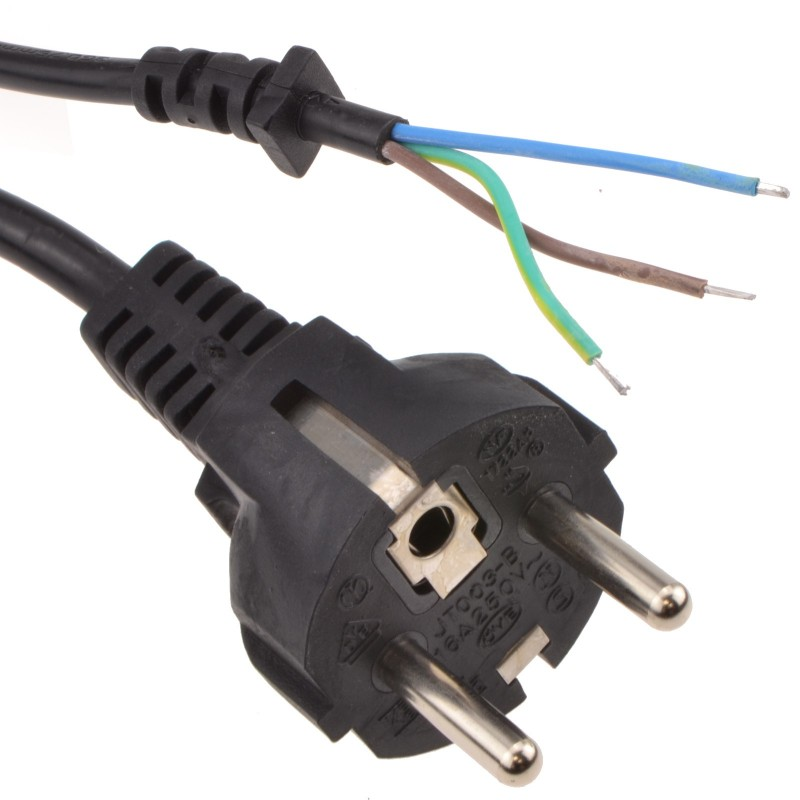
\includegraphics[width=0.4\textwidth]{07hw_specification/eletrical_wire}
	\caption{Plug to bare end wire 5 A.}
	\label{fig:eletrical_wire}
\end{figure}

The plug separates in three wires, which must be carefully connected to the power supply, as previously seen. These wires have a color pattern, as one shows in table \ref{table:color_pattern_wire}.

\begin{table}[H]
	\centering
	\begin{tabular}{|m{5cm}|m{6cm}|}
		\hline
		\textbf{Color pattern} & \textbf{Description}
		\\\hline\hline
		
		Brown wire & Power grid phase 230 V \ac{ac}
		\\\hline
		Blue wire & Power grid neutral
		\\\hline
		Green/Yellow wire & GND
		\\\hline
	\end{tabular}
	\caption{Color pattern on eletrical wires.}
	\label{table:color_pattern_wire}
\end{table}

In order to provide a lower voltage to power the Raspberry Pi and sensors, it is necessary to use a step down module, as the one shown in figure \ref{fig:step_down}, which can convert 12 V \ac{dc} to 5 V \ac{dc}. \cite{step_down}
 
\begin{figure}[H]
	\centering
	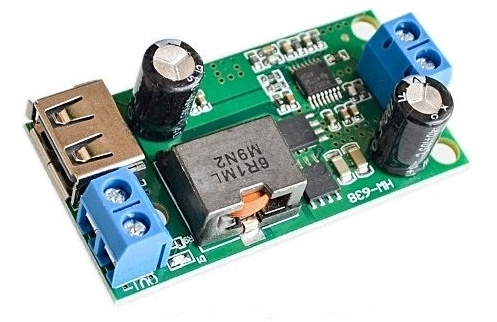
\includegraphics[width=0.5\textwidth]{07hw_specification/step_down}
	\caption{Step Down 9-38~V to 5~V / 5~A.}
	\label{fig:step_down}
\end{figure}

\paragraph*{Characteristics}
\begin{itemize}
	\item Input voltage 9-38 V;
	\item Output voltage 5 V / 5 A;
	\item Load capacity: 5 A;
	\item Maximum efficiency of 95 \%.
\end{itemize}

\begin{table}[H]
	\centering
	\begin{threeparttable}
	\begin{tabular}{|m{5cm}|m{6cm}|}
		\hline
		\textbf{Step Down Pinout} & \textbf{Description}
		\\\hline\hline
		
		VCC & Input voltage 9-38 V
		\\\hline
		GND & Input GND
		\\\hline
		USB & USB output 5 V / 5 A \tnote{*}
		\\\hline
		VOUT+ & Output 5 V / 5 A \tnote{*}
		\\\hline
		VOUT- & Output GND
		\\\hline
	\end{tabular}
	
	\begin{tablenotes}
		\small
		\item[*] This module provides 5 A for both output pins combined (USB and VOUT+).
	\end{tablenotes}
	\end{threeparttable}
	\caption{Step-Down Pinout Description.}
	\label{table:step_down_pinout}
\end{table}

\myparagraph{Connection scheme}
In table \ref{table:step_down_pinout} is shown the connection scheme for the step down. Keep in mind that the same power supply output 12 V \ac{dc} is connected directly to the lamp VCC and to the step down VCC.

\begin{table}[H]
	\centering
	\begin{tabular}{|m{5cm}|m{6cm}|}
		\hline
		\textbf{Step Down Pin} & \textbf{Connects to}
		\\\hline\hline
		
		VCC & Power supply Output +12 V \ac{dc}
		\\\hline
		GND & Power supply Output GND
		\\\hline
		USB & Raspberry Pi USB-C
		\\\hline
		VOUT+ & Sensors VCC
		\\\hline
		VOUT- & Sensors GND
		\\\hline
	\end{tabular}
	
	\caption{Connection scheme: Step Down.}
	\label{table:connect_power}
\end{table}

\myparagraph{Test Cases}
It is important to know how the step down works, and how it will behave upon certain events. In table \ref{table:test_step_down} are shown test cases to this module.

\begin{table}[H]
	\centering
	\resizebox{\columnwidth}{!}
	{
		\begin{tabular}{|m{3cm}|m{5cm}||m{5cm}|}
			\hline
			\textbf{Test Case} & \textbf{Expected Output} & \textbf{Real Output}
			\\\hline\hline
			Connect power supply to the power grid & Provide 12 V \ac{dc} & -
			\\\hline
			Connect step down to the power supply & Provide 5 V \ac{dc} & -
			\\\hline
		\end{tabular}
	}
	\caption{Test Cases: Step Down.}
	\label{table:test_step_down}
\end{table}
%**********************************************************
\subsection{Driver}
In order to control the lamp brightness through a GPIO pin from the Raspberry Pi, it's needed a driver circuit, as shown in figure \ref{fig:driver}. This circuit takes as input a \ac{pwm} signal, provided by the raspberry Pi, and also the power for the lamp, \(V_{CL}\), which comes directly from the power supply 12 V \ac{dc} output of the power module. The output of this circuit, the lamp voltage \(V_{L}\), is directly related to it's brightness, which one wants to control.

\begin{figure}[H]
	\centering
	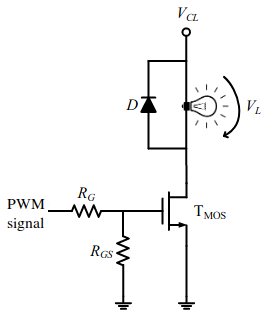
\includegraphics[width=0.5\textwidth]{07hw_specification/driver}
	\caption{Driver circuit to control lamp brightness.}
	\label{fig:driver}
\end{figure}

The \ac{pwm} signal only takes two values, 0 or 3,3 V, but its average value over time is varied, changing at high frequency the time intervals in which the transistor \(T_{MOS}\) is conducting (applied voltage 3,3 V) and at cutoff (applied voltage 0 V). So, as the \ac{pwm} duty cycle increases, the transistor conducts for more time, leading to an increase of \(V_{L}\), and, therefore, to an increase of the lamp brightness. In any case, the power dissipation in the transistor is very low, because of the rapid change between each transistor state, conducting (at saturation) or at cutoff.

\paragraph*{Characteristics}
\begin{itemize}
	\item Transistor MOSFET;
	\item Resistor \(R_{G}\) limits the current in the gate of the transistor;
	\item Resistor \(R_{GS}\) ensures that the gate is set to 0 potential when the circuit is turned off;
	\item Diode D, known as free-wheeling, provides a way to discharge the energy stored in the magnetic field of the inductive load, when the transistor turns off. For that reason, this diode must be fast;
\end{itemize}

In order to specify the components to be used, the following must be taken into account.

The temperature of the transistor (internal at the junction) must not exceed the maximum allowed by the manufacturer (typically 150 °C as in the case of STP60NF06, BUK453, BUZ90). In order for the transistor to be used without a heatsink, the internally dissipated power must not exceed 2~W (taking into account the typical thermal resistance of a TO-220 package, 60~°C/W and the ambient temperature of 30 °C). Considering that 50 \% of losses occur in conduction and 50  \% in switching (very vague approximation), the transistor can only dissipate 1 W in conduction and 1 W in switching. For an \(I_{DS}\) current of 2 A, the internal resistance (\(R_{DS}\) of MOSFET to \(V_{GS}\) voltage, \(I_{DS}\) current and operating temperature) will be a maximum of 250 m$\Omega$ (P = \(R_{DS}\).\(I_{DS2}\)).

Diode D should be fast and the MR852 is recommended.\linebreak

With this in mind, one can select the following components for the driver, as presented in table \ref{table:driver_components}.

\begin{table}[H]
	\centering
	\resizebox{\columnwidth}{!}
	{
		\begin{tabular}{|m{5cm}|m{6cm}|m{2.6cm}|}
			\hline
			\textbf{Driver Component} & \textbf{Product Name} & \textbf{Product Qty}
			\\\hline\hline
			
			\(T_{MOS}\) & BUK453 & 1
			\\\hline
			Diode D & MR852 & 1
			\\\hline
			Resistor \(R_{G}\) & Common; +-5 \% tolerance & 1
			\\\hline
			Resistor \(R_{GS}\) & Common; +-5 \% tolerance & 1
			\\\hline
		\end{tabular}
	}
	\caption{Driver components.}
	\label{table:driver_components}
\end{table}

\myparagraph{Connection scheme}
In table \ref{table:connect_driver} is shown the connection scheme for the driver circuit. (Remember figure \ref{fig:rasp_pinout} and table \ref{table:power_supply_pinout})

\begin{table}[H]
	\centering
	\begin{tabular}{|m{5cm}|m{6cm}|}
		\hline
		\textbf{Driver} & \textbf{Connects to}
		\\\hline\hline
		
		PWM Signal & Raspberry Pi PWMxxx Pinyyy
		\\\hline
		\(V_{CL}\) & Power supply Output +12 V \ac{dc}
		\\\hline
		GND & Power supply Output GND
		\\\hline
	\end{tabular}
	
	\caption{Connection scheme: Driver.}
	\label{table:connect_driver}
\end{table}

\myparagraph{Test Cases}
It is important to know how the driver works, and how it will behave upon certain events. In table \ref{table:test_driver} are shown test cases to this circuit.

\begin{table}[H]
	\centering
	\resizebox{\columnwidth}{!}
	{
		\begin{tabular}{|m{3cm}|m{5cm}||m{5cm}|}
			\hline
			\textbf{Test Case} & \textbf{Expected Output} & \textbf{Real Output}
			\\\hline\hline
			Apply 3,3 V to the transistor & Lamp at maximum bright & -
			\\\hline
			Apply 0 V to the transistor & Lamp off & -
			\\\hline
			Change \ac{pwm} signal & Variable lamp brightness & -
			\\\hline
		\end{tabular}
	}
	\caption{Test Cases: Driver.}
	\label{table:test_driver}
\end{table}

%**********************************************************
\subsection{Hardware review} %?????
% show hardware architecture with all protocols defined in
% each connection

\clearpage
\chapter{Software Specification}
%**********************************************************
\section{Local System}
%**********************************************************
\subsection{Task Overview}
One can define and describe briefly how the local system is implemented, making use of threads and processes. As one can see in figure \ref{fig:task_overview}, this system is composed by two processes: the main process and a daemon, used to read the sensors \textit{LDR} and \textit{LampFailureDetector}, \textit{dSensors}. As the \textit{PIR} sensor can be read through the use of an ISR, this sensor stays in the main process. The communication between the daemon and the main process is done via message queue.

\begin{figure}[H]
	\centering
	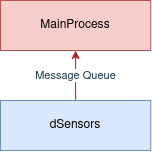
\includegraphics[width=.3\textwidth]{09sw_specification/task_overview}
	\caption{Inter-process Communication between Main Process and Daemon.}
	\label{fig:task_overview}
\end{figure}

\clearpage
One can list the tasks that compose the main process:
\begin{itemize}
	\item \textbf{tCamera:} acquire a camera frame; processes image and search for parking spots; verify the parking spot availability;
%	\item \textbf{tLampControl:} initializes PWM interface; controls the PWM applied to the lamp;
	\item \textbf{tLoraSend:} sends a message to the gateway, using the LoRa module;
	\item \textbf{tLoraRecv:} receives a message from the gateway, using the LoRa module;
	\item \textbf{tRecvSensor:} receives messages sent by the daemon, via message queue, regarding sensors information.
\end{itemize}

%**********************************************************
\subsection{Task Priority}

%**********************************************************
\subsection{Task Synchronization}
Real-time tasks share resources and services, and as such, should be prepared to await for the availability of these resources and services, like logical resources (buffers and data), physical resources, services like directory services, etc. In order to have coordinate access to shared resources and avoid race conditions, the kernel has resources that provide synchronization tools. 

\myparagraph{Condition Variables}

A condition variable is a task synchronization tool that can be used to block (wait) one or more threads, suspending its execution. The blocked threads are awakened when the condition variable is notified. The condition variables used are listed below.

\begin{itemize}
	\item \textbf{condCameraAcquire:} used to notify \textit{tCamera} that a camera sample period has elapsed;
	
%	\item \textbf{condNewPWM:} used to notify \textit{tLampControl} that a new PWM value for the lamp was defined;
	
	\item \textbf{condSend:} used to notify \textit{tLoraSend} that a new message is ready to be sent;
	
	
\end{itemize}

\myparagraph{Mutexes}

A mutex is a locking mechanism that provides mutual exclusion, supporting ownership and other protocols. A mutex is initially created in the unlocked state in which it can be acquired by a task. After being acquired, the mutex moves to the locked state. When the task releases the mutex, it returns to the unlocked state. The mutexes used are listed bellow.

\begin{itemize}
	\item \textbf{mutCamera:} mutex associated with the condition variable \textit{condCameraAcquire} to acquire a camera frame;
		
	\item \textbf{mutSend:} protects the message to be sent in \textit{tLoraSend}, which can be defined in multiple places;
	
	\item \textbf{mutComms:} protects LoRa communication, since it is half-duplex, so one can send or receive at a time; Used in \textit{tLoraSend} and \textit{tLoraRecv};
	
	\item \textbf{mutChangePWM:} protects the modification of PWM when defining a new PWM value for the lamp;
	
	
\end{itemize}

%\myparagraph{Semaphores}

\subsection{Task Communication}
%\myparagraph{Pipes}
%
%Pipe is an inter-process communication tool, that establishes a connection between two processes, such that the standard output from one process becomes the standard input of the other process. Pipe is one-way communication, i.e, we can use a pipe such that one process write to the pipe and the other process reads from the pipe. If a process tries to read before something is written to the pipe, the process is suspended until something is written.
%
%As previously stated, it's used a pipe to communicate between the \textit{dSensors} to the main process. In this way, the main process can know if something was detected by the sensors and provide a response to that.

\myparagraph{Message Queue}

A message queue is a linked list of messages stored within the kernel and identified by a message queue identifier. A message queue will be used to communicate between the main process and the \textit{dSensors}. In that way, the main process is agnostic to the cyclic reading necessary for the sensors \textit{LDR} and \textit{LampFailureDetector}, and is only informed when necessary, thorough the message queue.

%**********************************************************
\subsection{Class Diagrams}
\myparagraph{Class Camera}

In figure \ref{fig:classcamera} is shown the Camera class diagram, that defines a camera object.  For this project the camera is used to detect available parking spots in the lamppost vicinity, so this class defines the functions used to capture (\textit{captureFrame()}) and process (\textit{processFrame}) a camera frame. After the creation of the object, using the constructor \textit{Camera()}, the thread \textit{tCamera()} is executed every time the condition variable \textit{condCameraAcquire} is signaled, that happens every 2 minutes.

%This class defines all the functions that implicate the use of the camera device.

\begin{figure}[H]
	\centering
	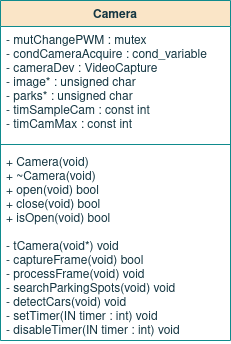
\includegraphics[width=.5\textwidth]{09sw_specification/classcamera}
	\caption{Class Diagram: Camera.}
	\label{fig:classcamera}
\end{figure}

\myparagraph{Class Lamp}

In figure \ref{fig:classlamp} is shown the Lamp class diagram, which defines a Lamp object. After creating the object, using the constructor \textit{Lamp()}, one can interact with it by changing the brightness, through the method \textit{setBrightness(lux)}, where \textit{lux} is a value from 0, lamp OFF, to 100, lamp at maximum brightness. Internally, this class uses a mutex, \textit{mutChangePWM} to protect the PWM value when using \textit{setBrightness} method. 

\begin{figure}[H]
	\centering
	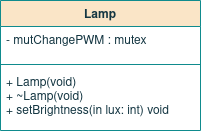
\includegraphics[width=.5\textwidth]{09sw_specification/classlamp}
	\caption{Class Diagram: Lamp.}
	\label{fig:classlamp}
\end{figure}

\myparagraph{Class Communications}

In figure \ref{fig:classcomm} is shown the Communications class diagram. This class defines an object Communication capable of establishing a LoRa communication with the gateway, through the use of the constructor \textit{Communication()}, and send messages through the use of \textit{Send(msg)}. It's used a vector of messages \textit{queued\_msgs} to store the message that's in the waiting list to be sent, in order to avoid the loss of a communication. To exchange messages are used two threads, \textit{tLoraSend} to send, and \textit{tLoraRecv} to receive, which makes use of task synchronization tools to ensure that sending and receiving don't occur at the same time, since the LoRa module in use is Half-Duplex.

\begin{figure}[H]
	\centering
	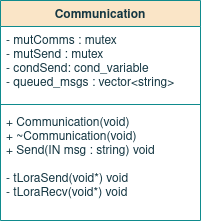
\includegraphics[width=.5\textwidth]{09sw_specification/classcomms}
	\caption{Class Diagram: Communications.}
	\label{fig:classcomm}
\end{figure}

%**********************************************************
\subsection{Flowcharts}
%\clearpage
\myparagraph{tCamera}

The task tCamera is responsible for acquire a frame from the Raspberry Pi Camera and to process it. It must analyze the returned frame, in order to detect empty parking spots. This thread uses the mutex \textit{mutCamera} to protect the condition variable \textit{condCameraAcquire}, that synchronizes the camera frame acquisition with the timer that defines the camera frame acquisition period, \textit{timSampleCam}.

Firstly, this thread initializes the camera device, sets the timer \textit{timSampleCam}, locks the mutex \textit{mutCamera} and goes to sleep mode, waiting for the conditon variable \textit{condCameraAcquire} to be signaled. This happens when a \textit{timSampleCam} period has elapsed and the thread wakes up. Now, one can capture a camera frame in order to process it, unlocking the mutex \textit{mutCamera}. A timer, \textit{timCamMax}, is setted to report the error if the image is taking too much time to being processed.

In the image processing part of the thread, if there aren't parking spots coordinates stored, then it is necessary to search for parking spots. After that, one can detect cars using the pre-trained model and the function \textit{detectCars} that detects cars in the image. If the coordinates of a detected car matches the coordinates of the parking spot, then one can assume that the parking spot is occupied. If the parking spot status has changed, then it is necessary to send this to the remote system, using the LoRa communication module.

\myparagraph{tRecvSensors}

This task, presented in figure \ref{fig:flow_trecv_sensors}, is responsible for receiving messages sent by the sensors daemon, through a message queue.

When the message queue is not empty, this task reads a message from the message queue and parses it, in order to find out which sensor was triggered and what action this system should take. For that, a list of commands may be defined:
\begin{itemize}
%	\item Lamp Max: the lamp brightness must be at its maximum (PWM=100);
	\item Lamp Min: the lamp must be at minimum bright level (PWM = \textit{MIN\_BRIGHT\_PWM});
	\item Lamp OFF: the lamp must be OFF (PWM=0);
	\item Lamp Fail: the lamp must be OFF, since there was a failure detected on the lamp.
\end{itemize}

\begin{figure}[H]
	\centering			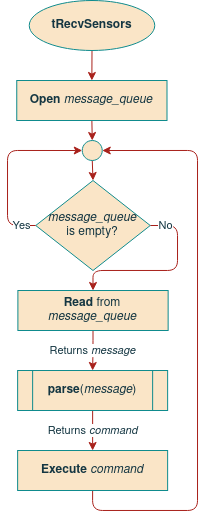
\includegraphics[width=.4\textwidth]{09sw_specification/trecvsensors}
	\caption{Main Process Flowchart: tRecvSensors.}
	\label{fig:flow_trecv_sensors}
\end{figure}

%**********************************************************
\clearpage
\myparagraph{Class Lamp Constructor and Destroyer}

This functions, presented in figure \ref{fig:flow_lampconstruct}, are responsible for initializing and destroying a Lamp object. First, in the constructor, which is the left side function, the PWM peripheral is initialized, then the mutex that is used to protect the change of PWM is also initialized. On the destroyer side, the opposite is done, by the terminating the PWM generation.

\begin{figure}[H]
	\centering	
	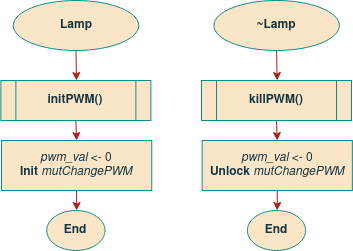
\includegraphics[width=.7\textwidth]{09sw_specification/lampconstruct}
	\caption{Class Lamp Flowchart: Constructor and Destroyer.}
	\label{fig:flow_lampconstruct}
\end{figure}

\myparagraph{setBrightness}

This function, presented in figure \ref{fig:flow_setbrightness}, is responsible for changing the PWM associated with the lamp, which is directly related to its brightness. Through \textit{setPWM(lux)} one can change the current lamp PWM to \textit{lux} value, being this an integer between 0 to 100. When the PWM is maximum, a timer is started that defines how much time the lamp is ON, \textit{LAMP\_ON\_TIMEOUT} in seconds, if there isn't another call of this function.

\begin{figure}[H]
	\centering	
	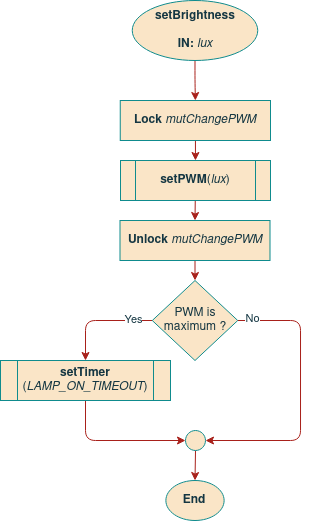
\includegraphics[width=.6\textwidth]{09sw_specification/lampsetbrightness}
	\caption{Class Lamp Flowchart: setBrightness.}
	\label{fig:flow_setbrightness}
\end{figure}


%**********************************************************
\clearpage
\myparagraph{Class Communication Constructor and Destroyer}

This functions, presented in figure \ref{fig:flow_commconstruct}, are responsible for initializing and destroying a Communication object. On the left side, the constructor, starts by initializing the LoRa communication, defining the frequency in which the device choosen previously operates, which is 433~MHz. Then the messages vector is cleared, the mutexes are initialized and the two threads responsible for the exchange of messages between the local system and the gateway are created. In the destroyer side, one has the opposite, where the LoRa communication is disabled and the threads are terminated.

\begin{figure}[H]
	\centering			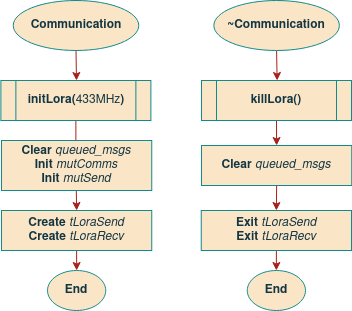
\includegraphics[width=.7\textwidth]{09sw_specification/commsconstruct}
	\caption{Class Communication Flowchart: Constructor and Destroyer.}
	\label{fig:flow_commconstruct}
\end{figure}

\myparagraph{tLoraSend}

This task is responsible for sending queued messages to the gateway, using LoRa communication. A conditional variable is used to wake this thread when there is a new message available to be sent.

When the vector \textit{queued\_msgs} is empty, then the task goes to sleep, waiting for the condition variable \textit{condSend} to notify this task. This happens when a new message is inserted into the messages vector, using \textit{Send(msg)} function, that will be later presented. After this, the mutex \textit{mutComms} is used to protect the communication, which due to the selected LoRa module is half-duplex, meaning that at a given moment, the device can be receiving or sending, not at the same time. Then, a message is popped from the messages vector, and sent to the gateway using the function \textit{LoraSend}. This continues to happen until the \textit{queued\_msgs} vector gets empty.

The flowchart for this task is presented in figure \ref{fig:flow_tlorasend}

\begin{figure}[H]
	\centering		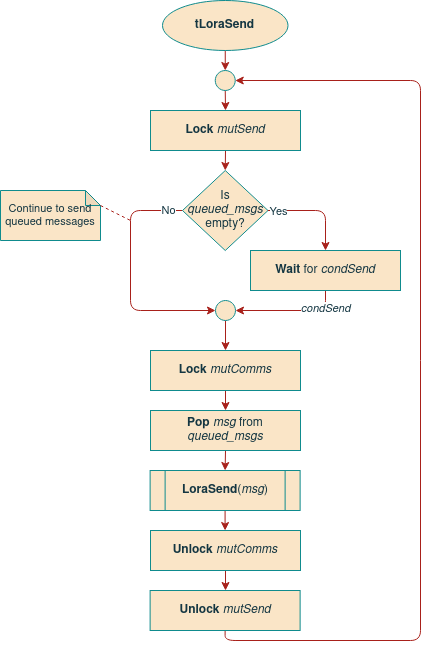
\includegraphics[width=.85\textwidth]{09sw_specification/commstlorasend}
	\caption{Class Communication Flowchart: tLoraSend.}
	\label{fig:flow_tlorasend}
\end{figure}


\myparagraph{tLoraRecv}

This task is responsible for receiving messages from the gateway, using LoRa communication.

When a message is received, using \textit{LoraReceive}, this is parsed and later, the respective command will be executed.

The flowchart for this task is presented in figure \ref{fig:flow_tlorarecv}

\begin{figure}[H]
	\centering		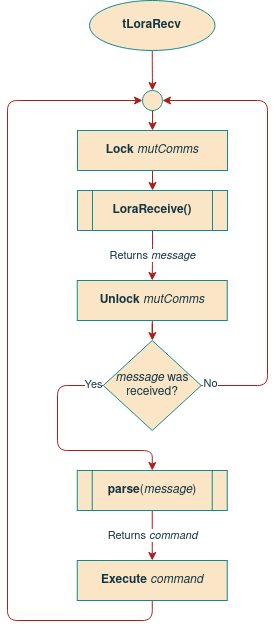
\includegraphics[width=.55\textwidth]{09sw_specification/commstlorarecv}
	\caption{Class Communication Flowchart: tLoraRecv.}
	\label{fig:flow_tlorarecv}
\end{figure}

\myparagraph{Send}

This function, presented in figure \ref{fig:flow_send}, is responsible for adding a new message, \textit{msg}, to the \textit{queued\_msgs} vector, and signal the condition variable \textit{condSend}, for the task \textit{tLoraSend} to send the message.

\begin{figure}[H]
	\centering	
	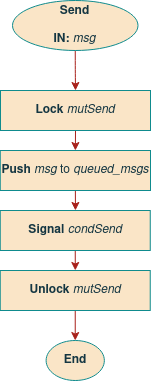
\includegraphics[width=.3\textwidth]{09sw_specification/commssend}
	\caption{Class Communication Flowchart: Send.}
	\label{fig:flow_send}
\end{figure}


% FLOWCHARTS SENSORS

\myparagraph{PirIsr}
The PIR sensor uses the GPIO of the Raspberry Pi in order to inform the system if there's movement in the surrounding area. In the afirmative case, it puts the high digital value on its output, and this can be used to generate an interrupt service routine, triggered on the rising edge of the output signal of the sensor. When this routine is executed, it locks the mutex \textit{mutChangePWM} and assign the \textit{PWM\_val} its maximum value, 100 \%, unlocking the mutex. Now, one needs to send the PWM value to the remote system through the LoRa communications, in order to be updated in the remote system. In the figure \ref{fig:pir_isr}, is represented the flowchart of the PirIsr function.

\begin{figure}[H]
	\centering
	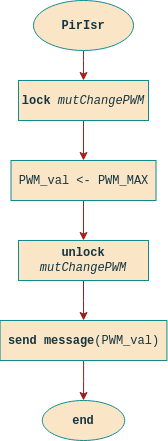
\includegraphics[width=.2\textwidth]{09sw_specification/pir_isr}
	\caption{PirIsr flowchart.}
	\label{fig:pir_isr}
\end{figure}

\myparagraph{LdrIsr}
The ambient light sensor, LDR, is used to determine when is time to turn on the lights, that is, when is night time and interfaces with the Raspberry Pi through I2C protocol communication. As the sun set or the sun rise is a relatively long time process, there's no need to keep checking the sensor output value all the time, so one can define a period to get the sensor value, \textit{LDR\_TIM}, that can be 10 minutes. In figure \ref{fig:ldr_isr} is shown the LDR sensor interrupt service routine, triggered by the timer overflow. When the timer period elapses, the illuminance value is calculated by the sensor. If this value is lower than the threshold value defined as good luminosity illuminance, GOOD\_LIGHT\_LUX, then the auxiliary variable, \textit{lightCon} is setted to high. In the next step, if the \textit{oldLightCon} variable (stores the last ambient light condition) is not equal to the auxiliary variable, then it is needed to change the \textit{oldLightCon} variable and send message to the process that controls the lamp PWM, through message queue. 

\begin{figure}[H]
	\centering
	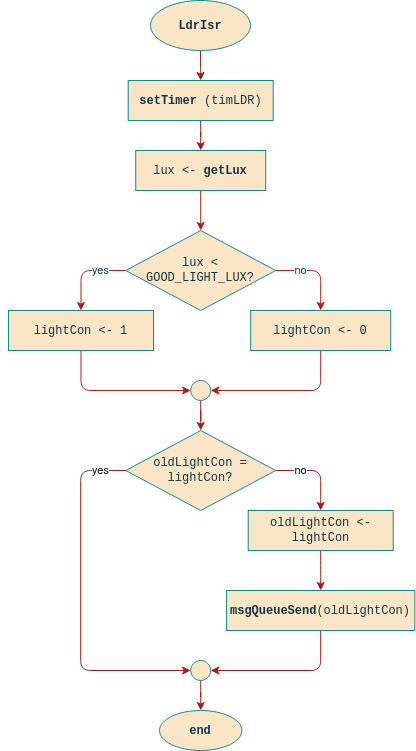
\includegraphics[width=.4\textwidth]{09sw_specification/ldr_isr}
	\caption{LdrIsr flowchart.}
	\label{fig:ldr_isr}
\end{figure}

\myparagraph{FailureDetectIsr}
In figure \ref{fig:fail_isr} is represented the FailureDetectIsr flowchart. Similarly to the PIR sensor, this routine is triggered on the rising edge of the output signal of the sensor. When the Failure detector detects that the lamp is broken, it puts the high digital value in its output, triggering this function. In this routine, the PWM is setted to 0 \% and are sent two messages through message queue: one to inform the process, that controls the lamp, to change the PWM value in the channel; and the other to notify the remote system that the lamp is broken, in order to update this status on the database.

\begin{figure}[H]
	\centering
	\includegraphics[width=.3\textwidth]{09sw_specification/fail_isr}
	\caption{FailureDetectIsr flowchart.}
	\label{fig:fail_isr}
\end{figure}

%**********************************************************
\subsection{Start-up Process}

%**********************************************************
\subsection{Shutdown Process}

%\myparagraph{tLampControl}
% uses: mutChangePWM; condNewPWM; pwm_val
% pwm_val is used in: PIR_sensor, CommandCb, LDR
% must define: MIN_BRIGHT_PWM; LAMP_ON_TIMEOUT
%This task is responsible for initializing and controlling the PWM peripheral used to control the lamp brightness. A mutex \textit{mutChangePWM} is used to protect the process of defining a new PWM value. 
%
%After initializing the PWM, this task goes to sleep, waiting for the condition variable \textit{condNewPWM} to notify this task. This happens when a new PWM value is defined into the variable \textit{pwm\_val}, in \textit{dReadSensors} or in a received command. Then, the lamp PWM is changed to the new value. 
%
%The lamp may have various levels of luminosity: for the lamp to be OFF, is applied PWM~=~0; for the lamp to be at a predefined minimum bright level, is applied PWM~=~\textit{MIN\_BRIGHT\_PWM}; for the lamp to be at maximum bright, this is, when the lamp must be ON, is applied PWM~=~100. So, since the lamp must stay ON a minimum amount of time out of a motion is detected or out of a request from the remote system to be ON, one needs to check if the new PWM is the maximum value. If so, that means that the lamp should continue with that PWM for a predefined time, defined by \textit{LAMP\_ON\_TIMEOUT}, in seconds.


%**********************************************************
\clearpage
\section{Gateway}
One can define the relationship between the tasks as follows, in figure \ref{fig:GwOverview}. The rule of the gateway is to receive LoRa messages and send the content in TCP-IP messages, or vice versa.

\begin{figure}[H]
	\centering
	\includegraphics[width=1\textwidth]{09sw_specification/Gateway/overview}
	\caption{Gateway Overview.}
	\label{fig:GwOverview}
\end{figure}

%**********************************************************
\subsection{Class Diagrams}
In figure \ref{fig:GwclassDiag} is represented the class diagram of gateway, \textit{CGateway}, which is the main class of the system, responsible for initializing the objects of each class listed below.

\begin{itemize}
	\item \textbf{CLoraComm:} manages the LoRa communications with the local systems, interfacing with the LoRa module; this class was already detailed previously;
	
	\item \textbf{CTCPclient:} manages the TCP-IP communication with the remote server;
\end{itemize}

\begin{figure}[H]
	\centering	\includegraphics[width=.68\textwidth]{09sw_specification/Gateway/cgateway/class}
	\caption{CGateway Class Diagram.}
	\label{fig:GwclassDiag}
\end{figure}

\myparagraph{Class CTCPclient}

In figure \ref{fig:TCPclientClass} is shown the CTCPclient class. This class defines a TCPclient capable of establishing a connection to a given remote server and to exchange messages to it, via TCP-IP. Like in the CLoraComm class, this class inherits from the class CCommunication.

\begin{figure}[H]
	\centering
	\includegraphics[width=.4\textwidth]{09sw_specification/Gateway/ctcpclient/class}
	\caption{Class Diagram: TCPclient.}
	\label{fig:TCPclientClass}
\end{figure}

%**********************************************************
\clearpage
\subsection{Task Overview}
One can define and describe briefly how the gateway is implemented, making use of threads and processes.

\begin{itemize}
	\item \textbf{tLoraRecv:} receives all messages from local systems, using LoRa communication;
	\item \textbf{tTCPRecv:} receives all messages from the remote server, using TCP-IP communication;	
	\item \textbf{CLoraComm::tSend:} sends all received messages from the remote server, in \textit{tTCPRecv}, to the local systems, using LoRa communication; 
	\item \textbf{CTCPclient::tSend:} sends all received messages from local systems, in \textit{tLoraRecv}, to the remote server, using TCP-IP communication;
\end{itemize}

%**********************************************************
\subsection{Task Priority}
The priority assignment diagram for the gateway is represented in figure \ref{fig:gwt_priority}.

\begin{figure}[H]
	\centering
	\includegraphics[width=0.6\textwidth]{09sw_specification/Gateway/priority}
	\caption{Gateway Priority Assignment Schematic.}
	\label{fig:gwt_priority}
\end{figure}

%**********************************************************
\subsection{Task Synchronization}

\myparagraph{Condition Variables}

The condition variables used in this system are listed below.

\begin{itemize}
	\item \textbf{CCommunication::condSend:} already detailed in the local system section; this condition variable is used indirectly by \textit{CTCPclient} and \textit{CLoraComm}.
\end{itemize}

\myparagraph{Mutexes}

The mutexes used in this system are listed bellow.

\begin{itemize}
	\item \textbf{CCommunication::mutComms} and \textbf{CCommunication::mutTxMsgs:} already detailed in the local system section; this mutexes are used indirectly by \textit{CTCPclient} and \textit{CLoraComm}.
\end{itemize}

%%**********************************************************
\subsection{Start-up Process}
In figure \ref{fig:bootGateway} is shown the start-up process for the gateway. When booting up, the gateway creates a CGateway object, initializing all needed members, and after that, runs until all the threads termination.

\begin{figure}[H]
	\centering		\includegraphics[width=.3\textwidth]{09sw_specification/Gateway/mainprocess}
	\caption{Start-Up Process: Gateway.}
	\label{fig:bootGateway}
\end{figure}

%**********************************************************
\clearpage
\subsection{Flowcharts}
%Each local system has a predefined ID, which may be presented in a physical label for an operator to use this information. When a local system is being installed, it will use it's predefined ID in all communications with the remote server until the operator registers the local system that's being installed, in the remote server. By doing this, the remote server assigns a new ID to the local system, which is then sent to the local system, for this to be used in further communications.

%*****************************
\myparagraph{CGateway Methods}

In figure \ref{fig:gwtCGatewayconstructor} is shown the \textit{CGateway} class constructor. With this, one can create a CTCPclient and a CLoraComm objects. After this the threads are created and both objects begin running their threads for receiving and sending messages.

\begin{figure}[H]
	\centering
	\includegraphics[width=.3\textwidth]{09sw_specification/Gateway/cgateway/constructor}
	\caption{Flowchart: CGateway constructor.}
	\label{fig:gwtCGatewayconstructor}
\end{figure}

\clearpage
This task, presented in figure \ref{fig:gwtLoraRecv}, is responsible for receiving all the packets sent by the local systems, through LoRa communication. When a message is received it is pushed into the TCP client list of queued messages, waiting to be sent to the remote server.

\begin{figure}[H]
	\centering
	\includegraphics[width=.5\textwidth]{09sw_specification/Gateway/cgateway/tlorarecv}
	\caption{Flowchart: CGateway tLoraRecv method.}
	\label{fig:gwtLoraRecv}
\end{figure}

\clearpage
This task, presented in figure \ref{fig:gwtTCPRecv}, is responsible for receiving the messages sent by the remote system to the local systems. Unlike the \textit{tsend} tasks, this thread never enters the sleep state because one can receive a message at any moment. If it is received a message, then one can push the message to the messages queue in CLoraComm, signaling its thread to send the message, via LoRa communication.

\begin{figure}[H]
	\centering
	\includegraphics[width=.5\textwidth]{09sw_specification/Gateway/cgateway/ttcprecv}
	\caption{Flowchart: CGateway tTCPRecv method.}
	\label{fig:gwtTCPRecv}
\end{figure}

%*****************************
\clearpage
\myparagraph{CTCPclient Methods}

A TCPclient can be created through the use of the constructor, shown in figure \ref{fig:TCPclientconstructor}. This connects to a given server, defined by the string \textit{host}, and to the port \textit{port}, via TCP-IP and initializes all the private members.

\begin{figure}[H]
	\centering
	\includegraphics[width=.36\textwidth]{09sw_specification/Gateway/ctcpclient/constructor}
	\caption{Class Diagram: CTCPclient constructor.}
	\label{fig:TCPclientconstructor}
\end{figure}

As in CLoraComm, this class must implement \textit{recvFunc} and \textit{sendFunc}, as they are pure virtual methods from CCommunication. 

In this class, one will use existent functions \textit{TCPReceive} and \textit{TCPSend} to implement TCP-IP communication, as shown in figures \ref{fig:TCPclientrecvfunc} and \ref{fig:TCPclientsendfunc}. This functions make use of socket associated with the TCP-IP established connection.

\begin{figure}[H]
	\centering
	\includegraphics[width=.35\textwidth]{09sw_specification/Gateway/ctcpclient/recvfunc}
	\caption{Flowchart: CTCPclient recvFunc method.}
	\label{fig:TCPclientrecvfunc}
\end{figure}

\begin{figure}[H]
	\centering
	\includegraphics[width=.35\textwidth]{09sw_specification/Gateway/ctcpclient/sendfunc}
	\caption{Flowchart: CTCPclient sendFunc method.}
	\label{fig:TCPclientsendfunc}
\end{figure}

%**********************************************************
\clearpage
\section{Remote System}
%**********************************************************
The remote system is responsible for the communication between the local systems and the internet. In this project, the internet is used to maintain a cloud database, so the remote system does the data bridge between the network of street lampposts and a cloud. As one can see in figure \ref{fig:rs_overview}, the remote system is composed by the main process and a daemon process \textit{dServerSend}. The main process may be composed of a server and varoius clients, being the messages from each client received and processed in this process. The messages are sent to the clients in the daemon process \textit{dServerSend}. The communication between the two processes is done using message queues, so when a command is received and successfully parsed, the main process sends the command output to the daemon using the message queue.

\begin{figure}[H]
	\centering
	\includegraphics[width=.6\textwidth]{09sw_specification/RS/overview}
	\caption{Inter-process Communication between Main Process and Daemon.}
	\label{fig:rs_overview}
\end{figure}

%**********************************************************
\subsection{Class Diagram}
In figure \ref{fig:rs_classDiag} is represented the class diagram of the remote system. The class \textit{CTCPServer} is the main class of the system, that initializes the objects of each class, listed below. 

\begin{itemize}
	\item \textbf{CTCPServer:} main class, responsible for creating the server, the client objects, each time a client connects to the server and for sending the messages to the clients;
	\item \textbf{CClient:} client class, stores the clients information and receives their messages;
	\item \textbf{CDataBase:} provides an interface between the server and the database.

\end{itemize}

\begin{figure}[H]
	\centering
	\includegraphics[width=.9\textwidth]{09sw_specification/RS/ClassDiagram}
	\caption{Remote System Class Diagram.}
	\label{fig:rs_classDiag}
\end{figure}

%****************************
\myparagraph{Class CTCPServer}

This class is responsible for creating the server, using \textit{createServer} function, allowing multiple clients to connect and send them messages, with the thread \textit{tSend}. When a client connects to the server, this class creates a new instance of the class \textit{CClient}. Each client can be of a different type of device like website, mobile application or gateway. The clients are assigned to their respective list of clients that are \textit{webSList}, \textit{appList} and \textit{gatewayList}, respectively. To do the interface with the database, this class also has an instance of the class database. In figure \ref{fig:CTCPServer}, one can see the class \textit{CTCPServer} diagram.

\begin{figure}[H]
	\centering
	\includegraphics[width=.6\textwidth]{09sw_specification/RS/CTCPServer/CTCPServer}
	\caption{Class Diagram: CTCPServer.}
	\label{fig:CTCPServer}
\end{figure}

%****************************
\myparagraph{Class CClient}

The class \textit{CClient}, represented in figure \ref{fig:CClient}, is responsible for storing information about a client connected to the server, like the \textit{cmdList}, a vector that stores all the client commands list and \textit{clientSock}, and also for receiving messages from the clients in the thread \textit{tRecv}. The \textit{clientSock} has information about the client connected such as its \textit{state}, its client identification (\textit{index}), its name in \textit{clientName}, its file descriptor \textit{sockFd} and its type of client \textit{type}, that can be: \textit{GATEWAY}; \textit{WEBSITE}; or \textit{APPLICATION}.

\begin{figure}[H]
	\centering
	\includegraphics[width=.6\textwidth]{09sw_specification/RS/CClient/CClient}
	\caption{Class Diagram: CClient.}
	\label{fig:CClient}
\end{figure}

%****************************
\myparagraph{Class CDataBase}

This class diagram is shown in figure \ref{fig:CDataBase}, and is responsible for implement the interface between the server and the database, having for that a pointer to a database of type \textit{MYSQL}. To interact with the database, the server must first prepare a query, using the function \textit{prepareQuery}, and can update or get data from the database, using the prepared query and the functions \textit{updateData} and \textit{getData}, respectively.

\begin{figure}[H]
	\centering
	\includegraphics[width=.5\textwidth]{09sw_specification/RS/CDataBase}
	\caption{Class Diagram: CDataBase.}
	\label{fig:CDataBase}
\end{figure}

%**********************************************************
\subsection{Task Overview}
One can define and describe briefly how the remote system is implemented, making use of threads and processes. 

\begin{itemize}
	\item \textbf{tSend:} sends a message to a client;
	\item \textbf{tRecv:} receives a message from the clients.
\end{itemize}

%**********************************************************
\subsection{Task Priority}
As the two threads \textit{tRecv} and \textit{tSend} run in two different processes, daemon process and main process, respectively, one needs to define the threads priority assignment for the two processes. The priority assignment diagram for the remote system main process is represented in figure \ref{fig:rsMainPrio} and for the daemon process is shown in the figure \ref{fig:rsDaemonPrio}. 

\begin{figure}[H]
	\centering
	\includegraphics[width=.5\textwidth]{09sw_specification/RS/MainPrio}
	\caption{Remote System Main Process Priority Assignment.}
	\label{fig:rsMainPrio}
\end{figure}

\begin{figure}[H]
	\centering
	\includegraphics[width=.5\textwidth]{09sw_specification/RS/DaemonPrio}
	\caption{Remote System Daemon Process Priority Assignment.}
	\label{fig:rsDaemonPrio}
\end{figure}

%**********************************************************
\subsection{Task Synchronization}
As seen before, to have coordinate access to shared ressouces and services and avoid race conditions, the kernel has resources that provide synchronization between the tasks. 

\myparagraph{Mutexes}

The mutexes used for the remote system are listed bellow.

\begin{itemize}
	\item \textbf{CTCPServer::mutComms:} mutex used to protect the messages sending;
	\item \textbf{CClient::mutComms:} mutex used to protect the messages receiving.
\end{itemize}

\subsection{Task Communication}
\myparagraph{Message Queues}

In order to the main process communicate with the daemon process and send messages to the clients, one can use a message queue, named \textit{msgqComms}, that send the messages from the main process to the daemon process, containing the messages to be sent from the server to the clients.

%**********************************************************
\subsection{Flowcharts}
\myparagraph{CTCPServer}

In figure \ref{fig:ServerConst} is represented the constructor of the \textit{CTPCServer} class, that is responsible for creating the class variables, initializing the mutex and for creating the thread \textit{tSend} and the server socket in the port passed by argument.

\begin{figure}[H]
	\centering
	\includegraphics[width=.26\textwidth]{09sw_specification/RS/CTCPServer/ServerConst}
	\caption{Flowchart: CTCPServer Constructor.}
	\label{fig:ServerConst}
\end{figure}

The function that creates a server socket for a maximum number of clients, \textit{maxClient}, is represented in figure \ref{fig:RSCreateServer}. This function initiates a server socket with the IPv4 protocol connection.

\begin{figure}[H]
	\centering
	\includegraphics[width=.3\textwidth]{09sw_specification/RS/CTCPServer/CreateServer}
	\caption{Flowchart: CTCPServer createServer.}
	\label{fig:RSCreateServer}
\end{figure}

In figure \ref{fig:RSInit}, is shown the method that creates the thread \textit{tSend} with the priority \textit{tprio} passed by argument.

\begin{figure}[H]
	\centering
	\includegraphics[width=.26\textwidth]{09sw_specification/RS/CTCPServer/Init}
	\caption{Flowchart: CTCPServer Init.}
	\label{fig:RSInit}
\end{figure}

The function \textit{run} is responsible for waiting for the termination of the thread \textit{tSend}.

\begin{figure}[H]
	\centering
	\includegraphics[width=.26\textwidth]{09sw_specification/RS/CTCPServer/run}
	\caption{Flowchart: CTCPServer run.}
	\label{fig:RSrun}
\end{figure}

In figure \ref{fig:RSsend} is represented the thread \textit{tSend}, which is responsible for sending a message to a client. It reads the messages to be sent in a message queue and send them to the recipient client.

\begin{figure}[H]
	\centering
	\includegraphics[width=.95\textwidth]{09sw_specification/RS/CTCPServer/send}
	\caption{Flowchart: CTCPServer tSend.}
	\label{fig:RSsend}
\end{figure}

%**********************************
\myparagraph{CClient}

In figure \ref{fig:ClientConst} is represented the constructor of the \textit{CClient} class. Every time a client connects to the server, it creates an instance of this class, passing by argument, the information about the client to initialize the \textit{clientSock} variable. The constructor also creates the command list that the type of client can execute, \textit{cmdList}, and the thread \textit{tRecv}.

\begin{figure}[H]
	\centering
	\includegraphics[width=.20\textwidth]{09sw_specification/RS/CClient/ConsClient}
	\caption{Flowchart: CClient Constructor.}
	\label{fig:ClientConst}
\end{figure}

The command list, \textit{cmdList} varies with the type of client:

\begin{itemize}
	\item \textbf{Mobile Application:} 
		\begin{itemize}
			\item Get;
			\item Update;
			\item Delete.
		\end{itemize}
	
	\item \textbf{Web Site:}
		\begin{itemize}
			\item Get.			
		\end{itemize}
	
	\item \textbf{Gateway:}
		\begin{itemize}
			\item Get;
			\item Update;
		\end{itemize}

\end{itemize}


%**********************************************************
\subsection{Start-up Process}

%**********************************************************
\subsection{Shutdown Process}


%**********************************************************
\clearpage
\section{Database}
The database's logic diagram is presented in figure \ref{fig:database_er}.

\begin{figure}[H]
	\centering	
	\includegraphics[width=1\textwidth]{09sw_specification/DataBase}
	\caption{Database Entity-Relationship Diagram.}
	\label{fig:database_er}
\end{figure}


%\myparagraph{Logic Model}

%**********************************************************
\clearpage
\section{\ac{gui} Layouts}
In this section it is presented the \ac{gui} layouts, where the users can interact with the system.

\myparagraph{Mobile Application}

The mobile application is used by the operator, in order to manage the network of lampposts that is assigned to him. 

The first step is to login the system, so he has to insert is credentials \textit{ID Operator} and \textit{Password}, provided by the company. The login layout is shown in figure \ref{fig:login}.

\begin{figure}[H]
	\centering	
	\includegraphics[width=.3\textwidth]{10gui_layouts/App/login}
	\caption{Mobile Application Layout: Login.}
	\label{fig:login}
\end{figure}

If the login was successful, then the operator can select one of this operations: \textit{Add New Lamppost}, \textit{Modify Lamppost} or \textit{Consult Lamppost Network}, as shown in figure \ref{fig:selectOperation}. The operator can also logout of his account.

\begin{figure}[H]
	\centering	
	\includegraphics[width=.3\textwidth]{10gui_layouts/App/selectOperation}
	\caption{Mobile Application Layout: Select Operation.}
	\label{fig:selectOperation}
\end{figure}

If he clicks on the \textit{Add New Lamppost} option, then he is redirected to the layout represented in figure \ref{fig:addNewLamppost}, where he can add a new lamppost to the network, inserting all the information about the location of the post or use his mobile device actual location. 

\begin{figure}[H]
	\centering	
	\includegraphics[width=.3\textwidth]{10gui_layouts/App/addNewLamppost}
	\caption{Mobile Application Layout: Add New Lamppost.}
	\label{fig:addNewLamppost}
\end{figure}

If the option chosen was the \textit{Modify Lamppost}, in order to change the lamppost status, he can insert the location of the post or use his mobile device actual location, as seen in figure \ref{fig:modifyLamppost}.

\begin{figure}[H]
	\centering	
	\includegraphics[width=.3\textwidth]{10gui_layouts/App/modifyLamppost}
	\caption{Mobile Application Layout: Modify Lamppost.}
	\label{fig:modifyLamppost}
\end{figure}

If the lamppost selection was valid, then the layout represented in figure \ref{fig:acceptModify} appears, to the operator confirm that he wants to update the lamppost status.

\begin{figure}[H]
	\centering	
	\includegraphics[width=.3\textwidth]{10gui_layouts/App/acceptModify}
	\caption{Mobile Application Layout: Modify Lamppost Confirmation.}
	\label{fig:acceptModify}
\end{figure}

On the other hand, if the operator selects the option \textit{Consult Lamppost Network}, the network information will appear like shown in figure \ref{fig:consultNetwork}, where the red point are lampposts with a broken lamp and the green points are the lampposts with no lamp problems.

\begin{figure}[H]
	\centering	
	\includegraphics[width=.3\textwidth]{10gui_layouts/App/consultNetwork}
	\caption{Mobile Application Layout: Consult Lamppost Network.}
	\label{fig:consultNetwork}
\end{figure}

\myparagraph{Web Site}



%**********************************************************
% TOOLS, COTS and THIRD PARTY LIBRARIES
\section{Tools}

\begin{itemize}
	\item \textbf{Buildroot:} Tool to configure and generate the Raspberry Pi Kernel image;
	\item \textbf{C/C++:} Programming language used to develop local system and remote system core;
	\item \textbf{Qt Creator:} Cross-platform IDE used for the Mobile Application development;
	\item \textbf{HTML:} Programming language chosen for the WebSite development;
	\item \textbf{Python:} Programming language chosen for the Haar cascade training stage;
	\item \textbf{MySQL:} Relational database management system used for the remote server database;
%	\item \textbf{MQTT:}
\end{itemize}

\section{COTS}

\begin{itemize}
	\item \textbf{POSIX Threads API:} Used for thread creation and management;
	\item \textbf{OpenCV API:} Used for image capture and processing;
	\item \textbf{Qt API:} Used for the GUI;
	\item \textbf{RaspiCam API:} C++ API for using Raspberry camera with/without OpenCv;
	\item \textbf{Cloudant API:} IBM cloud service that executes transactions in databases; ???
	\item \textbf{Google Cloud SQL:} Google Cloud service that allows for immutable data storage and retrieval;
\end{itemize}

\section{Third-Party Libraries}

\begin{itemize}
	\item \textbf{Light Sensor (TSL258x) Device Driver:} Open-source device driver used for interfacing with the luminosity sensor \cite{code_tsl};
	\item \textbf{LoRa SX1278 Library:} An Arduino open-source library for sending and receiving data using LoRa radios \cite{sx1278_lib}. This is implemented to the Arduino board, but it will be adapted to the Raspberry Pi 4 Model B.
\end{itemize}



% ---------- SYSTEM IMPLEMENTATION ----------
\clearpage
\chapter{Implementation}
%**********************************************************
\section{Tools Setup}
Before doing the system configuration it is necessary to first setup all of the used tools, as will be next presented.

%**********************************************************
\subsection{Git}
In order to make collaboration easier, allowing change by multiple people to all be merged into one source, Git will be used. Git is the most commonly used version control system. Before using it, it is necessary to do the correct setup as shown bellow.
\begin{lstlisting}
$ sudo apt install git
$ git config --global user.name "John Doe"
$ git config --global user.email johndoe@example.com
$ git config --global core.editor subl
$ cd ~
$ git clone git@github.com:ESRGgroup9/slipad.git
\end{lstlisting}

With this steps, Git is installed in a local machine, username and user email is defined alongside with the default core editor. After this, one can clone the repository for this project, created in GitHub, by executing line 6.

%**********************************************************
\subsection{Buildroot}
Buildroot is a simple, efficient and easy-to-use tool used to generate this project's embedded Linux system, through cross-compilation. The steps in order to install Buildroot in a local machine is shown bellow.

\begin{lstlisting}
$ cd ~
$ mkdir buildroot
$ cd buildroot
$ wget https://buildroot.org/downloads/buildroot-2021.02.5.tar.gz
$ tar xzf buildroot-2021.02.5.tar.gz
$ cd buildroot-2021.02.5
\end{lstlisting}

After the installation is done, one can do the base configurations, essential to the support the rest of the configurations.
\begin{lstlisting}
$ make raspberrypi4_defconfig
$ make menuconfig
$ make xconfig
$ make 
$ make clean
\end{lstlisting}

The first command is used to configure a kernel image for the Raspberry Pi 4, as it does the necessary configurations regarding hardware handling along with fetching some board specific packages. Then with the second and third commands, one can generate the graphic interface seen in figure \ref{fig:menuconfig}, presenting several sub-menus. 

\begin{figure}[H]
	\centering	
	\includegraphics[width=.74\textwidth]{11configs/menuconfig}
	\caption{Buildroot menuconfig.}
	\label{fig:menuconfig}
\end{figure}

%**********************************************************
\subsection{OpenCV}

\begin{lstlisting}
$ cd ~/buildroot/buildroot-2021.02.5/output/build/opencv3-3.4.13/buildroot-build
$ cmake-gui
$ cmake .
$ make -j8
$ sudo make install
\end{lstlisting}

%**********************************************************
\subsection{Qt Creator}

The Qt Creator IDE was used to create an application that is used by the operator to interact with the system. The IDE instalation is done by downloading the open-source online installer present on the official site, in the download page \cite{qt_creator}. In the figure \ref{fig:qt_instalation} is shown all the packages installed for this IDE.

\begin{figure}[H]
	\centering	
	\includegraphics[width=.80\textwidth]{11configs/qt_instalation}
	\caption{Qt Creator: Instalation.}
	\label{fig:qt_instalation}
\end{figure}

Since one is deploying the application to an Android device, it was necessary to install and configure the Android Studio and SDK tools \cite{android_studio}, and also Android NDK \cite{android_ndk} in the Qt Creator. To install the Android Studio run \verb|<path-to-android-studio>/android-studio/bin/studio.sh|. Next, one needs to configure the platform of the Android Studio accordingly to the android phone version. The Android NDK must be the \verb|r23| version, and the Qt creator configure the packages missing.

It is also necessary to install a Java SE Development (JDK) \cite{java}. The JDK version shouldn't be the latest and the installed one was the version 11. Now, run \verb|<path-to-android-studio>/android/tools/bin/sdkmanager --licenses| in order to accept the licenses. 

At last, the \verb|QT -> Tools -> Options -> Devices -> Android|, sould look like shown in figure \ref{fig:qt_config}.

\begin{figure}[H]
	\centering	
	\includegraphics[width=.80\textwidth]{11configs/qt_config}
	\caption{Qt Creator: Configuration.}
	\label{fig:qt_config}
\end{figure}

%**********************************************************
\subsection{MySQL}
In order to have a fully managed database service to deploy cloud-native applications as MySQL, one has to firstly install it properly, as shown bellow.

\begin{lstlisting}
$ sudo apt-get install libmysqlclient-dev
\end{lstlisting}

First time runnning \verb|mysql|, one can create a strong password for \verb|mysql| access. After that, one can login into \verb|mysql| by typing:

\begin{lstlisting}
$ mysql -u root -p
\end{lstlisting}

%**********************************************************
\subsection{PHP}
In order to fetch data from the remote server database to the website that will present available parking spots, one uses PHP, which must first be configured. The following commands must be executed so that one gets a PHP client and PHP with MySql.

\begin{lstlisting}
$ sudo apt install php7.4-cli
$ sudo apt install php-mysqli
\end{lstlisting}

Knowing that fetching data from a remote database envolves secret keys, such as servername, username, port number, database password, it is usefull to have a \verb|.env| file which will contain all of them. In order to load those variables into the website index file one needs to setup \verb|phpdotenv| following the steps bellow. \cite{phpdotenv}

\begin{lstlisting}
$ sudo apt install composer
$ composer install
$ composer require vlucas/phpdotenv
\end{lstlisting}

%**********************************************************
\subsection{Google Maps Credentials}
In order for the website to present the parking spaces at a given location in a map, one uses Google Maps API. In order to generate a Google API key, one needs to go to Google API Console \cite{googleapi} and:

\begin{enumerate}
	\item Create a \textbf{new project};
	\item In API Manager go into \textbf{Library} and select \textbf{Google Maps Javascript API};
	\item Select the created project to enable APIs;
	\item Enable API;
	\item In API Manager go into \textbf{Credentials} and in \textbf{Create Credentials} click \textbf{Create API key}	
\end{enumerate}

After this steps, one may retrieve the generated key and use it within website source file. Make sure that this does not leak since it is a secret key that it is not meant be shared.

%**********************************************************
\clearpage
\section{System Configuration}
\label{systemConfig}

In the Buildroot, using \verb|make menuconfig| one can use a graphic interface (as previously shown in figure \ref{fig:menuconfig}) to select packages and change configurations in order to create a custom linux image.\\

Under \verb|Target-Packages| select:
\begin{itemize}
%	\item \verb|Development tools|, select:
%	\begin{itemize}
%		\item \verb|git|
%	\end{itemize}
	
	% *****************************************************************************
	\item \verb|Networking applications|, select:
	\begin{itemize}
		\item \verb|arp-scan|: scan the network of a certain interface for alive hosts;
		\item \verb|arptables-legacy|: set up and maintain the tables of ARP rules;
		\item \verb|dhcpcd|: open source DHCP client;
		\item \verb|dropbear|: small SSH server which will let us log in remotely;
	\end{itemize}
	
	% *****************************************************************************
	\item \verb|Hardware Handling|
	\begin{itemize}
		\item \verb|spi-tools|: tools needed to use SPI. Used for LoRa module communication;
		\item \verb|i2c-tools|: tools needed to use I2C. Used for light sensor module, TSL2581;
		\item \verb|rpi-userland|: Used to detect camera hardware;
	\end{itemize}
	
	% *****************************************************************************
	\item \verb|Libraries|, select:
	\begin{itemize}
		% *******************************
		\item \verb|Hardware Handling|
		\begin{itemize}
			\item \verb|bcm2835|: C library for Raspberry Pi user programs;
			\item \verb|libv4l|: select \verb|v4l-utils tools|: API for real time video capture;
		\end{itemize}
		
		% *******************************
		\item \verb|Graphics|
		\begin{itemize}
			\item \verb|OpenCV3|: select \verb|jpeg support|, \verb|png support|, \verb|v4L support|, \verb|videoio|, \verb|highgui|, \verb|imgcodecs|, \verb|imgproc|, \verb|v4l support|: Used for image capturing and processing;
		\end{itemize}
	\end{itemize}

	% *****************************************************************************
	\item \verb|Audio and Video Applications|, select:
	\begin{itemize}
		\item \verb|v4l2grab|: utility for grabbing JPEG images;
	\end{itemize}
	% *****************************************************************************
	
\end{itemize}

%**********************************************************
\clearpage
\section{Image Generation}
After all the necessary tools, packages and configurations are done, one needs to finally create the Linux custom image, that will run on the Raspberry Pi.

\begin{lstlisting}
$ cd ~/buildroot/buildroot-2021.02.5/
$ make
\end{lstlisting}

After that one can copy the image into the SD card, that will go into the Raspberry Pi. For that one can use the linux \verb|dd| command. \cite{dd}

\begin{lstlisting}
$ sudo dd if=./output/images/sdcard.img of=/dev/sdb
\end{lstlisting}

With this command, one must define the input file, \verb|if|, which is the linux image, and the output file, \verb|of|, which is the SD card, being in this example named \verb|sdb|.


%**********************************************************
%\clearpage
\section{System Initialization}
The Buildroot generates the boot configuration, in the \verb|/boot/config.txt| file that contains system configuration parameters that are read when the system boots from the microSD card, and that would traditionally be edited and stored using a BIOS. \cite{configtxt} The listing \ref{lst:configtxt} shows the boot configuration file. For this project, one added the parameter in line 24, in order to enable the I2C device, the parameters in lines 26 and 27, to activate the camera.

\begin{lstlisting}[caption={/boot/config.txt file.}, label={lst:configtxt}]
# We always use the same names, the real used variant is selected by
# BR2_PACKAGE_RPI_FIRMWARE_{DEFAULT,X,CD} choice
start_file=start.elf
fixup_file=fixup.dat

kernel=zImage

# To use an external initramfs file
#initramfs rootfs.cpio.gz

# Disable overscan assuming the display supports displaying the full resolution
# If the text shown on the screen disappears off the edge, comment this out
disable_overscan=1

# How much memory in MB to assign to the GPU on Pi models having
# 256, 512 or 1024 MB total memory
gpu_mem_256=100
gpu_mem_512=100
gpu_mem_1024=100

# fixes rpi (3B, 3B+, 3A+, 4B and Zero W) ttyAMA0 serial console
dtoverlay=miniuart-bt

dtparam=i2c_arm=on 		# enable i2c

start_x=1             	# enable camera
gpu_mem=128           
\end{lstlisting}

%**********************************************************
\subsection{Init Scripts}
\verb|/etc/init.d| is a directory containing initialization and termination scripts for changing init states. File names in this directory are of the form \verb|[SK]nn<init.d filename>|, where \verb|S| means start this job, \verb|K| means kill this job, and \verb|nn| is the relative sequence number for killing or starting the job. \cite{initScript} For this reason, one must create a script, with name started by \verb|S|, inside \verb|/etc/init.d| in the Raspberry Pi, using for that, \verb|vi|.

In order to guarantee that each program is running after the system boots up, its necessary to create the respective init scripts, following the procedure detailed in listing \ref{lst:initScript}.

\begin{lstlisting}[caption={Procedure for creating an init script, named Sscript\_name}, label={lst:initScript}]
$ cd /etc/init.d
$ vi S<scriptName>.sh
$ chmod +x S<scriptName>.sh
\end{lstlisting}

The local system has the init script detailed bellow, in listing \ref{lst:lsScript}. This script must insert all necessary device drivers in order to correctly execute the local system's daemon, dSensors, and the main process. 

\begin{lstlisting}[caption={Init script for local system.}, label={lst:lsScript}]
#!/bin/sh

# Inserting i2c-tools
modprobe i2c-bcm2835
modprobe i2c-dev

# Inserting PIR DDriver
insmod /etc/pir.ko

# Inserting lampf DDriver
insmod /etc/lampf.ko

# Run local system's daemon sensor and main process
/etc/dSensors.elf &
/etc/localSys.elf
\end{lstlisting}

The gateway system has the init script detailed in listing \ref{lst:gatScript}. The gateway, \verb|gateway.elf| is connected via TCP-IP to the remote system. Therefore one can set the gateway to connect to \verb|10.42.0.1|, which is the network address of remote system in the same network as the gateway, in port \verb|5000|.

\begin{lstlisting}[caption={Init script for Gateway system.}, label={lst:gatScript}]
#!/bin/sh

etc/gateway.elf 10.42.0.1 5000
\end{lstlisting}

The remote system also has an init script, as shown in listing \ref{lst:rsScript}. This is responsible for running the website PHP server \cite{phpserver} and running the remote system in port \verb|5000|.

\begin{lstlisting}[caption={Init script for remote system.}, label={lst:rsScript}]
#!/bin/sh

# run website PHP server
php -S localhost:8000 -t ~/slipad/remoteSystem/website/ &

# run remote system
~/slipad/remoteSystem/bin/remoteSystem.elf 5000

\end{lstlisting}

%**********************************************************
\clearpage
\section{Device Drivers}
\subsection{tsl2581}
%.config - Linux/arm 5.10.1 Kernel Configuration
%> Device Drivers > Industrial I/O support > Light sensors
%
%-> TAOS TSL2580, TSL2581 and TSL2583 light-to-digital converters
%
%cat /lib/modules/5.10.1-v7l/modules.dep | grep tsl
In order to insert the \verb|tsl2581| device driver, available on the Linux kernel (\cite{code_tsl}) one needs to execute a series of steps.\\

Firstly, one needs to add a new entry on the Raspberry Pi device tree, regarding the \verb|tsl2581|. For that, one needs to change the Device tree Source file (.dts) for the Raspberry Pi, named \verb|bcm2711-rpi-4-b.dts|. This will be later compiled into a device tree binary (.dtb), when creating an image using Buildroot, which will be later passed by the boot loader to the operating system kernel. \cite{dtb}

\begin{lstlisting}
$ cd ~/buildroot/buildroot-2021.02.5/output/build/linux-custom/arch/arm/boot/dts
$ nano bcm2711-rpi-4-b.dts
\end{lstlisting}

At the end of the file, before \verb|__overrrides__|, the following code must be added, where \verb|reg| is the I2C address of the device. \cite{tsl2583_txt} 

\begin{lstlisting}
&i2c1 {
	status = "okay";
	
	tsl2581@29 {
		compatible = "amstaos,tsl2581";
		reg = <0x29>;
	};
};
\end{lstlisting}

For the Raspberry Pi, in the \verb|/boot/config.txt| file, one must enable \verb|i2c1| with a \verb|dtoverlay|, by adding the line of code shown next.
\begin{lstlisting}
dtoverlay=i2c1
\end{lstlisting}

When booting the Raspberry Pi, one must insert the \verb|tsl2581| device driver, but before that, some modules must be added using \verb|modprobe|.

This is an I2C based sensor, which uses the \ac{iio} interface. In order to provide the \ac{iio} API, needed in the device driver to be used, it is necessary to enable the \ac{iio} kernel subsystem, \verb|industrialio|. To enable the I2C bus, one must load the \verb|i2c-bcm2835| module. \cite{i2c_bcm2835}\\

After that, one can insert the \verb|tsl2581| device driver, \verb|ldr.ko|.

\begin{lstlisting}
$ modprobe industrialio
$ modprobe i2c-bcm2835
$ insmod ldr.ko
\end{lstlisting}

After the device driver insertion, one can use it to communicate with the sensor in order to acquire the ambient luminosity. For that, a “single” on-demand read can be issued by user-space directly by reading \linebreak \verb|/sys/bus/devices/iio:device/in_<type><index>_raw|. In this case, the \verb|read_raw()| callback should handle basically all the steps necessary to get the required measurement. \cite{read_tsl}
%**********************************************************
\subsection{PIR}

%**********************************************************
\clearpage
\section{LoRa communication}
LoRa communication was implemented by deriving a third-party software from Arduino. \cite{sx1278_lib} Using \verb|bcm2835| C library one was able to control all the needed GPIO and SPI functions. \cite{bcm2835} \cite{bcmspi}

By reading the LoRa module SX1278 documentation \cite{sx1278}, (page 80) one is able to find the figure \ref{fig:sx1278_spi}. The SPI interface gives access to the configuration register via a synchronous full-duplex protocol. One of three access modes to the registers is used - SINGLE access. In this mode:
\begin{itemize}
	\item \textbf{Write access:} an address byte followed by a data byte is sent;
	\item \textbf{Read access:} an address byte is sent and a read byte is received;
\end{itemize}

\begin{figure}[H]
	\centering	
	\includegraphics[width=1\textwidth]{12implementation/sx1278_spi}
	\caption{SPI Timing Diagram (single access).}
	\label{fig:sx1278_spi}
\end{figure}

A transfer is always started by the NSS pin going low. MISO is high impedance when NSS is high. MOSI is generated by the master on the falling edge of SCK and is sampled by the slave on the rising edge of SCK. MISO is generated by the slave on the falling edge of SCK. Both data to be transmitted and that has been received are stored in a configurable \ac{fifo} device. It is accessed via the SPI interface and provides several interrupts for transfer management. (Page 66, \cite{sx1278})
\\
In listing \ref{lst:lorasingletx} one can see LoRa single transfer function, which sends two bytes to the slave. 

\clearpage
\begin{lstlisting}[caption={LoRa single transfer.}, label={lst:lorasingletx}]
// set NSS pin low. Begin transfer
digitalWrite(_ss, LOW);

bcm2835_spi_transfer(address);
response = bcm2835_spi_transfer(value);

// set NSS pin high. Stop transfer
digitalWrite(_ss, HIGH);
\end{lstlisting}

By default, the device is configured at power up so that half of the available memory is dedicated to receive
(\verb|RegFifoRxBaseAddr| initialized at address 0x00) and the other half is dedicated for  (\verb|RegFifoTxBaseAddr| initialized at address 0x80). Therefore, when one wants to perform a transmit to the device, the address is always above \verb|0x80|. On the other hand, when one wants to perform a reading, the address is bellow \verb|0x80|. With that in mind one can use bit-masking to define the address for the operation, where, \verb|reg_addr| is the SX1278 register one wants to access:

\begin{itemize}
	\item \textbf{Read:} \verb|address = reg_addr & 0x7f| and \verb|value = 0x00|. The \verb|response| variable is the response from the slave;
	
	\item \textbf{Write:} \verb+address = reg_addr | 0x80+ and \verb|value| is the value to be written to the given address. \verb|response| is not used.
\end{itemize}

A LoRa message is defined by the class \verb|LoRaMsg| having the attributes shown in listing \ref{lst:loramsg}.

\begin{lstlisting}[caption={LoRa message.}, label={lst:loramsg}]
int recvAddr;     	// receiver address
int sendAddr;     	// sender address

int msgID;        	// message ID
size_t msgLength; 	// message length
string msg;       	// message
\end{lstlisting}

In listing \ref{lst:lorasend} is shown the main core of LoRa send function. This sends a series of attributes in each message, regarding destination address, sender address, message ID, message length and the message itself.

\begin{lstlisting}[caption={LoRa send function.}, label={lst:lorasend}]
beginPacket();

// add destination address  
write(destination);
// add sender address
write(localAddress);
// add message ID
write(msgCount);
// add message length
write(msg.length());
// add message
write(msg);

endPacket();
\end{lstlisting}

The function which implements LoRa receive, receives all of the attributes sent in the function above. Also it does some additional verifications to ensure communication integrity. The destination address in the message is compared to the local address of the device receiving the message, in order to avoid messages being mistakenly read. Besides that, one checks if the received message length matches the supposed length, by comparing the received message length to the message field regarding the message length.

In order to define LoRa status before a send/receive operation, a class is defined, as presented in listing \ref{lst:loraerr}.
 
\begin{lstlisting}[caption={LoRaError enum class.}, label={lst:loraerr}]
enum class LoRaError
{
	MSGOK = 0,  	// Message OK
	ENOADDR,		// Local address not defined
	ENOMSGR,    	// No message received
	ENOTME,     	// Message received is not for this device
	EBADLMSG    	// Message received lengths does not match
};
\end{lstlisting}

%**********************************************************
\clearpage
\section{PWM control}
In order to control the lamp, a PWM signal is used. For that, one can use \verb|bcm2835| library to control a PWM channel, producing the desired PWM signal at the selected GPIO pin. \cite{bcmpwm}

Considering that the clock which drives the PWM channels, \verb|clock|, is 54 MHz, and the lamp will operate at 50 Hz, \verb|freq|.

\[ RANGE = \frac{clock}{clock_{div} * freq} \]

Using a clock divider of 16, $clock_{div}$, one gets \verb|RANGE = 67500|. The variable \verb|RANGE| defines the maximum range of the PWM output, as shown in listing \ref{lst:pwmconfig}. One used \verb|PWM_CHANNEL 0|.

\begin{lstlisting}[caption={PWM configuration.}, label={lst:pwmconfig}]
// Set the output pin to Alt Fun 5, to allow PWM channel 0 to be output there
bcm2835_gpio_fsel(PWM_PIN, BCM2835_GPIO_FSEL_ALT5);
// set clock divider
bcm2835_pwm_set_clock(BCM2835_PWM_CLOCK_DIVIDER_16);
//CTL reg
bcm2835_pwm_set_mode(PWM_CHANNEL, 1, 1);
//RNG1/2 reg
bcm2835_pwm_set_range(PWM_CHANNEL, RANGE);
\end{lstlisting}

One can set the PWM pulse ratio to emit to \verb|RANGE|, where the duty cycle, \verb|duty| a value from 0 to 1, controls the PWM output ratio as a fraction of the range as shown in listing \ref{lst:pwmset}.

\begin{lstlisting}[caption={PWM set duty cycle.}, label={lst:pwmset}]
bcm2835_pwm_set_data(PWM_CHANNEL, (duty*RANGE));
\end{lstlisting}

%**********************************************************
\clearpage
\section{Luminosity Sensor}
\label{section:lumSensor}
As specified before, in order to know when to turn on/ off the lamp, it is used a luminosity sensor, the TSL2581. This module uses the I2C communication protocol to interface with the Raspberry Pi, being implemented based on a third-party software \cite{tsl2581_code}. As for the LoRa communication, one used the bcm2835 C library to communicate with the sensor module by I2C. \cite{bcmpiic}

From the theoretical foundations, one knows that the TSL2581 module uses a data line, SDA, to send and receive data, and a clock signal line, SCL, to synchronize the communication with the master device.

The sensor datasheet \cite{TSL2581_DS} shows that for the command code byte is used the \textit{Command Register} of the TSL2581, that is composed by:

\begin{itemize}
	\item \textit{CMD} bit: set to '1' when one wants to select the \textit{COMMAND} register;
	\item \textit{TRANSACTION} two bits: selects type of transaction to follow in subsequent data transfers, read/ write (R/W) mode and the special function register. For '00', select the I2C writing mode. For '10', selects the I2C reading mode which supports the read block protocol. For 11, select the special function register. 
	\item \textit{ADDRESS} five bits: when the \textit{TRANSACTION} field selects the R/W mode, then this field selects the bus address of the slave; when the \textit{TRANSACTION} field is set to '11', this field specifies a special command function.
\end{itemize}	

\myparagraph{I2C Address}

This module has three 7-bit address, as shown in table \ref{table:tsl_address}, and one can select one of them. By default, the \textit{ADDR state} register is set to FLOAT, so this device address in the I2C bus is the 0x39.

\begin{table}[H]
	\centering
	\begin{tabular}{|m{3cm}|m{3cm}|}
		\hline
		\textbf{ADDR State} & \textbf{Address}
		\\\hline\hline
		VCC & 0x49
		\\\hline
		FLOAT & 0x39
		\\\hline
		GND & 0x29
		\\\hline
	\end{tabular}
	
	\caption{TSL2581 I2C addresses.}
	\label{table:tsl_address}
\end{table}

\myparagraph{TSL2581 Initialization}

After connecting the device in the I2C bus, one should configure its registers before reading the value from its two ADC channels. In the listing \ref{lst:tslConfig} is shown the TSL2581 device initialization. First, one needs to configure the I2C bus, using the \verb|DEV_ModuleInit| function, passing, by argument, the device address of the light sensor, \verb|ADDR_FLOAT| (0x39, default). Using the \verb|CONTROL| register, one can power on the device, that puts all registers to their default value, enabling the R/W transactions. As the day-night transition is slow, one does not need to read the luminosity value much frequently, so one can define the maximum integration time (688,5 ms). It is also important to define the gain of the sensor. This sensor supports gains of 1, 8, 16 or 111. For indoor tests, it was used a gain of 16, but in a real outdoor model, it must be used a gain of 1.

\begin{lstlisting}[caption={TSL2581 Initialization.}, label={lst:tslConfig}]
if(DEV_ModuleInit(ADDR_FLOAT)==1)
	return false;

IIC_Write(COMMAND_CMD | CONTROL,CONTROL_POWERON);	// power on

IIC_Write(COMMAND_CMD | TIMING, INTEGRATIONTIME_688MS);  	// 688,5 ms
IIC_Write(COMMAND_CMD | CONTROL, ADC_EN | CONTROL_POWERON); // Every ADC cycle generates interrupt
IIC_Write(COMMAND_CMD | INTERRUPT, INTR_INTER_MODE);		// TEST MODE
IIC_Write(COMMAND_CMD | ANALOG, GAIN_16X);					// GAIN = 16
\end{lstlisting}

\myparagraph{Read Luminosity Values}

When the device is configured, one can read the luminosity values of the module channels. The TSL2581 has two channels: 

\begin{itemize}
	\item Channel 0: Value of visible and infrared light;
	\item Channel 1: Value of infrared light.
\end{itemize}

The listing \ref{lst:tslRead} presents the code that reads the channel 0 values, as for the channel 1 values, it is the same procedure. The lower byte is read out first using the \verb|DATA0LOW| register and next the higher byte, using the \verb|DATA0HIGH| register. Then, one combine them into a 16-bit variable as seen in the line 3.

\begin{lstlisting}[caption={TSL2581 Channel 0 read.}, label={lst:tslRead}]
DataLow = IIC_Read(COMMAND_CMD | TRANSACTION | DATA0LOW); 	// read channel 0 low byte
DataHigh = IIC_Read(COMMAND_CMD | TRANSACTION | DATA0HIGH);	// read channel 0 high byte
Channel_0 = 256 * DataHigh + DataLow ;
\end{lstlisting}

This values should be now converted to the luminous intensity. First, one needs to scale the value using the formula presented in the listing \ref{lst:tslscale}.

\begin{lstlisting}[caption={TSL2581 Channel 0 scaling.}, label={lst:tslscale}]
// scale the channel values
channel0 = (Channel_0 * chScale0) >>  CH_SCALE;
\end{lstlisting}

After scaling, it is calculated the ratio between channel 0 and channel 1 using the formula shown in listing \ref{lst:tslscale}.

\begin{lstlisting}[caption={TSL2581 ratio calculation.}, label={lst:tslratio}]
ratio1 = (channel1 << (RATIO_SCALE + 1)) / channel0;
ratio = (ratio1 + 1) >> 1; // round the ratio value
\end{lstlisting}

After calculate the multiple of the relative channel using the formulas given in the datasheet, one can export the current luminous intensity through the code presented in listing \ref{lst:tslCalc}, where lux is the final luminosity value. 

\begin{lstlisting}[caption={TSL2581 luminosity value calculation.}, label={lst:tslCalc}]
temp = ((channel0 * b) - (channel1 * m));
temp += (1 << (LUX_SCALE - 1));			// round lsb (2^(LUX_SCALE-1))
//  temp = temp + 32768;
lux_temp = temp >> LUX_SCALE;			// strip off fractional portion
\end{lstlisting}

%**********************************************************
\clearpage
\section{Database}
As previously stated, this system's database is developed using MySql. One can create a file, \verb|slipad.sql| to have the queries needed to create the database. Analysing the two main entities of the database, \verb|lamppost| and \verb|location|, one can see its implementation in listing \ref{lst:locationLamppost}.

\begin{lstlisting}[language=SQL, caption={Queries to create tables location and lamppost.}, label={lst:locationLamppost}]
DROP TABLE IF EXISTS `location`;
CREATE TABLE `location`(
	`id` INTEGER AUTO_INCREMENT,
	`latitude` DECIMAL(8,6) NOT NULL,
	`longitude` DECIMAL(9,6) NOT NULL,
	`post_code` CHAR(8) NOT NULL,
	`street_name` CHAR(50) NOT NULL,
	CONSTRAINT `UC_Coords` UNIQUE (`latitude`,`longitude`),
	PRIMARY KEY(`id`),
	FOREIGN KEY(`post_code`) REFERENCES `region`(`post_code`)
		ON UPDATE CASCADE
);

DROP TABLE IF EXISTS `lamppost`;
CREATE TABLE `lamppost`(
	`id` INTEGER,
	`address` INTEGER UNIQUE NOT NULL,
	`status` ENUM('FAIL', 'OFF', 'ON', 'MIN') DEFAULT('OFF'),
	`gateway_sd` INTEGER DEFAULT(-1),
	PRIMARY KEY(`id`),
	FOREIGN KEY(`id`) REFERENCES `location`(`id`)
		ON UPDATE CASCADE
);
\end{lstlisting}

In table \verb|location| there are a set of attributes needed to identify a particular location. Each location instance is directly connected with the existence of a lamppost. That way, the primary key for the lamppost table references the primary key from \verb|location|, which is the location \verb|id|.

Each lamppost is connected to the remote system, and that way to the database, through a gateway. For that reason, each lamppost instance needs to contain the socket file descriptor of the TCP connection established by the gateway that is connected to that lamppost (local system).\\

As in lamppost table, in table \verb|parking_space| each row is linked to a unique lamppost, which is connected to a unique location. Considering that the number of vacants in each parking space is initialized as zero, there is only the need of creating a parking space by defining its \verb|id|. For that reason, a trigger is used to insert a parking spot, in table \verb|parking_space|, after an insertion in \verb|lamppost|, using the id of the inserted lamppost as the id of the parking space. In listing \ref{lst:triggerinspark} it shown the implementation of the trigger in question.

\begin{lstlisting}[language=SQL, caption={Trigger to insert a parking spot after lampost insert.}, label={lst:triggerinspark}]
DELIMITER $$

DROP TRIGGER IF EXISTS insert_parking$$
CREATE TRIGGER insert_parking
	AFTER INSERT ON lamppost
	FOR EACH ROW
	BEGIN
		INSERT INTO parking_space(id) VALUES(NEW.id);
END$$

DELIMITER ;
\end{lstlisting}

One can execute all the queries in \verb|slipad.sql| in order to create the database by login into MySql and typing the command:
\begin{lstlisting}
mysql> source ~/slipad/database/slipad.sql;
\end{lstlisting}

After this, one should see the result shown in figure \ref{fig:showtables}, by typing the command \verb|show tables;|.

\begin{figure}[H]
	\centering	
	\includegraphics[width=0.3\textwidth]{13tests/database/showtables}
	\caption{Database: created tables}
	\label{fig:showtables}
\end{figure}


\subsection{Populating the database}
In order to populate the database faster, one used the queries format shown bellow, in listing \ref{lst:populatedb}.

\begin{lstlisting}[language=SQL, caption={Queries examples to populate database.}, label={lst:populatedb}]
INSERT INTO operator(id, name, password) VALUES
(NULL, 'Jonh', 'pass');

INSERT INTO region(post_code, operator_id, parish, county, district) VALUES
('9999-999', 1, 'Azurem', 'Guimaraes', 'Braga');

INSERT INTO location(id, latitude, longitude, post_code, street_name) VALUES
(1, 41.447986, -8.300469, '4800-045', 'Alameda Dr. Alfredo Pimenta');

INSERT INTO lamppost(id, address) VALUES
(1, 0xa2);

\end{lstlisting}

%**********************************************************
\section{Parking spots detection}
As previously stated before, the parking spots detection algorithm is based on OpenCv API. First one needs to capture a frame using the Raspberry Pi camera and store it, as shown in listing \ref{lst:captureframe}. 

\begin{lstlisting}[language=C, caption={Capture and Store frame from Camera.}, label={lst:captureframe}]
// read frame into lastFrame
camDev.read(lastFrame);

// write image to path
imwrite(IMAGE_PATH, lastFrame);
\end{lstlisting}

To capture the frame, one used the \ac{v4l} API and calibrated the camera parameters using the code present in listing \ref{lst:calibrateCamera}, in order to get a clear image from the camera. 

\begin{lstlisting}[language=C, caption={Capture and Store frame from Camera.}, label={lst:calibrateCamera}]
camDev.set(CAP_PROP_FRAME_WIDTH , FRAME_W); // 640
camDev.set(CAP_PROP_FRAME_HEIGHT, FRAME_H); // 480
camDev.set(CAP_PROP_BRIGHTNESS, CAM_BRIGHTNESS); // 20
camDev.set(CAP_PROP_CONTRAST, CAM_CONTRAST); // 0
camDev.set(CAP_PROP_SATURATION, CAM_SATURATION); //10

system("v4l2-ctl --set-ctrl=auto_exposure=0");
system("v4l2-ctl --set-ctrl=iso_sensitivity=4");
system("v4l2-ctl --set-ctrl=auto_exposure_bias=18");
system("v4l2-ctl --set-ctrl=exposure_time_absolute=1000");
system("v4l2-ctl --set-ctrl=exposure_dynamic_framerate=1");
system("v4l2-ctl --set-ctrl=white_balance_auto_preset=7");

system("v4l2-ctl --set-ctrl=sharpness=30");
\end{lstlisting}

When there is a image from the empty parking spots, one can identify the number of parking spots available for that lamppost. For that, it was used an algorithm that detect rectangles in an image since a parking spot shape is a rectangle. First, we apply the Gaussian blur to the image, in order to filter the image noise. Then, one searches for squares in every colour plane of the image, starting for mixing the channels an try several threshold levels with the canny edge detection function. After dilate the image to remove the holes between edge segments, one can find contours and store them in a list of 2D points. In the end, it is verified if the contours are between a defined size and if they don't overlap another rectangles. If the answer is affirmative, then contour is added to the park coordinates in the image held in the vector \verb|parkCoords|. In the listing \ref{lst:getOutline}, is shown the algorithm that detects parking spots in an image.

\begin{lstlisting}[language=C, caption={Parking Spots Detection.}, label={lst:getOutline}]
// apply gaussian
GaussianBlur(frame, gaussian, Size(7, 7), 0);

Canny(gray0, gray, 0, thresh, 5);
		
// find contours and store them all as a list
findContours(gray, contours, RETR_LIST, CHAIN_APPROX_SIMPLE);
	
// test each contour
for( size_t i = 0; i < contours.size(); i++ )
{
	addPark(contours[i]);
}
\end{lstlisting}

When one have the the parking spot outline, it is ready to detect if the parking spot is empty or vacant, using for that, the algorithm that detect objects from OpenCv using a Haar Cascade classifier, \verb|detectMultiScale|. It was used a pre-trained classifier to detect cars. If the centre of the detected car is near the centre of the parking spot than it means that the parking spot is occupied. In listing \ref{lst:detectCars}, is shown the algorithm that determines if the parking spots are empty or occupied. 

\begin{lstlisting}[language=C, caption={Empty Parking Spots Detection.}, label={lst:detectCars}]
vector<Point> rect = getRectPoints(features[f]);
	
// Is the car over the parking spot?
//  The center of the car match with the center of the parking spot?
int pos = isOverlapp(rect);
if( pos != -1 )
{
	vacantsNum--;
	// park unavailable
	parkStatus[pos] = 0;
}
\end{lstlisting}

%**********************************************************
\clearpage
\section{Website}
The website will present to the user the location and the number of available parking spots in a map. Since the website needs to know the informations about the lampposts network, PHP is used, to fetch data from the database. HTML is used to design the body of the website. That way, one will have a source file, named \verb|index.php|.

Firstly, using \verb|dotenv|, third-party software \cite{phpdotenv}, one loads the secret variables regarding the database connection, from the \verb|.env| file which contains the secret variables definitions, with the format shown in listing \ref{lst:dotenv}.

\begin{lstlisting}[language=php, caption={.env file example.}, label={lst:dotenv}]
SERVER=servername
USERNAME=username
PASSWORD='password'
DATABASE=database
\end{lstlisting}

Using \verb|$_ENV['var']| one can load \verb|var| from \verb|.env| file, into a variable in \verb|index.php|. After all necessary variables are loaded one can connect to the database using \verb|mysqli_connect|, as shown in listing \ref{lst:phpwebsite} Then, a query is made to the database, retrieving all lamppost information of where their number of vacants in the respective parking spaces are greater than zero.

\begin{lstlisting}[language=php, caption={Create PHP connection to the database.}, label={lst:phpwebsite}]
<?php
// load secret variables from .env
require_once 'vendor/autoload.php';
$dotenv = Dotenv\Dotenv::createImmutable(__DIR__);
$dotenv->load();

$servername=$_ENV['SERVER'];
$username=$_ENV['USERNAME'];
$password=$_ENV['PASSWORD'];
$database=$_ENV['DATABASE'];

// connect to database
$con = mysqli_connect($servername, $username, $password, $database);

// execute query
// ...
?>
\end{lstlisting}

Entering the HTML section of the \verb|index| file, one will follow Google Maps documentation \cite{mapsdoc} in order to add a Google Map with several markers, relative to lampposts locations, using the HTML body presented in listing \ref{lst:website}. Lines 18 to 21 refer to the Google API script, that in order to use it, one needs to insert the Google API key, previously generated, in \verb|YOUR_API_KEY| (line 19). This is a secret key that should only be defined in \verb|.env| file. 

\begin{lstlisting}[language=HTML, caption={Website: Adding a map with a marker.},label={lst:website}]
<!DOCTYPE html>
<html>
	<head>
		<style>
			#map {
				height: 400px;
				width: 10%;
			}
		</style>
	</head>
	<body>
		<h3>My Google Maps Demo</h3>
		
		<!--The div element for the map -->
		<div id="map"></div>
		
		<!-- Async script executes immediately -->
		<script async defer
		src="https://maps.googleapis.com/maps/api/js?key=YOUR_API_KEY&callback=
		initMap">
		</script>
	</body>
</html>
\end{lstlisting}

In the Google API script, one can see that it has a parameter called \verb|callback| that is set to \verb|initMap|, which will be tried to be loaded. That way, its necessary to add another \verb|script| tag in HTML, where one will have to define \verb|function initMap()|. Inside \verb|initMap()| one must set a new Google Map object in order to have a map displayed.

Having the map displayed, then one needs to add markers of where the parking spaces available are. That way, a function \verb|addMarker| is created using JavaScript, as shown in listing \ref{lst:addmarker}. This function receives the marker coordinates, \verb|props.coords| and text message, \verb|props.content| which will pop up in a \verb|InfoWindow| when the user clicks on the marker.

\begin{lstlisting}[language=HTML, caption={Website: Function for adding a marker.},label={lst:addmarker}]
// Add Marker Function
function addMarker(props){
	var marker = new google.maps.Marker({
		position:props.coords,
		map:map,
	});

	// Check content
	if(props.content){
		var infoWindow = new google.maps.InfoWindow({
			content:props.content
		});
		
		marker.addListener('click', function(){
			infoWindow.open(map, marker);
		});
	}
}
\end{lstlisting}

By executing the command \verb|php -S localhost:8000|, inside the directory where \verb|index.php| is, one can open it in the browser and check the final result, presented in figure \ref{fig:websiteWindow}.

\begin{figure}[H]
	\centering	
	\includegraphics[width=1\textwidth]{13tests/website/website}
	\caption{Website: window.}
	\label{fig:websiteWindow}
\end{figure}

Whenever any of the markers is clicked on, the respective parking space informations are displayed, as shown in figure \ref{fig:websiteMarker}.

\begin{figure}[H]
	\centering	
	\includegraphics[width=.4\textwidth]{13tests/website/websiteMarker}
	\caption{Website: Marker info window.}
	\label{fig:websiteMarker}
\end{figure}


\section{Mobile Application}

The mobile application interacts with the database via TCP/IP via local server. When the application is executed, it tries to connect to the server held, in this case in the IP \verb|192.168.1.114| and port \verb|5000|. In the listing \ref{lst:appConnection}, is represented the connection establishment with the server. After the connection is done, the application sends a message to the server, indicating the type of its device, in this case, an application (\verb|TYPE;2|).

\begin{lstlisting}[language=C, caption={Mobile Application: Connection to the server.}, label={lst:appConnection}]
CTCPclient tcp(string("192.168.1.114"), 5000);

int main(int argc, char *argv[])
{
	// connect to tcp server
	ret = tcp.connect();
	if(ret == 0)
	{
		qDebug() << "Connection established";
		break;
	}
	
	err = errno;
	if(err != ECONNREFUSED)
	{
		// unexpected connection error
		qDebug() << "[CGateway::connect] Connect failed: " << err;
	}
	
	// send type to remote system
	QString msg = "TYPE;2";	
	do
	{
		ret = tcp.send(msg.toStdString());
		err = errno;
	} while((ret == -1) && (err == EAGAIN));
	
	// Handle errors
	...
}
\end{lstlisting}

When the operator tries to add a lamppost to the database, the application has to get the actual GPS location from the mobile phone. In the listing \ref{lst:appLocation} is shown the code that obtains the location from a \verb|QGeoPositionInfoSource|, connecting first to it and then start receiving updates in a period of 1 second. When the application wants to access the location, it can be done using the \verb|source->lastKnownPosition().coordinate()|, that return the last known position coordinates.

\begin{lstlisting}[language=C, caption={Mobile Application: Obtain GPS coordinates.}, label={lst:appLocation}]
source = QGeoPositionInfoSource::createDefaultSource(this);
if ( source )
{
	// conect to GPS
	connect(source, SIGNAL(positionUpdated(QGeoPositionInfo)), 
			this, SLOT(positionUpdated(QGeoPositionInfo)));
	// start updating localization
	source->startUpdates();
}
\end{lstlisting}

When a button is pressed in a window, it is executed the correspondent trigger function and when one wants to show other windows, it must be defined one instance of the window and call the \verb|show| function. In listing \ref{lst:appButton}, one can see an example of a button pressed call back function that invokes another window.

\begin{lstlisting}[language=C, caption={Mobile Application: Button trigger function.}, label={lst:appButton}]
void menu::on_add_new_released()
{
	addMenu = new addLamp(this);
	addMenu->show();
}
\end{lstlisting}

%**********************************************************
%\section{Local System}
%
%%**********************************************************
%\section{Gateway}
%
%%**********************************************************
%\section{Remote System}


% ---------- BIBLIOGRAPHY ----------
\bibliographystyle{IEEEtran}
\bibliography{References}

\end{document}